%!TEX root = ../thesis.tex

\subsection{Sweepcycle algorithm}
\thispagestyle{plain}
\label{ss:sweep}
The first step of our algorithm is executing a sweepcycle algorithm inspired by the sweepcycle algorithm by Fusy \cite{Fusy2006}. We use $\C$ to indicate the current sweep cycle. We shrink $\C$ by updating it with certain interior paths.
One of the nicest things about the regular edge labeling we produce is Lemma \ref{lm:sweep:NoTwoSplitsAboveEachOther} which will turn out to be very useful throughout the rest of the algorithm. This lemma states that most interior paths we can't have the fan handle of a large splitfan after a split vertex on a so-called bottom path. \fxnote{Q: These are all words the reader doesn't know yet. How to explain?}

During the algorithm we maintain several invariants on $\C$. The first three are equivalent to those imposed by Fusy. The final invariant is new and allows is us to prove Lemma \ref{lm:sweep:NoTwoSplitsAboveEachOther}.

\begin{invariants}
  \itemsep=-4pt

  \item \label{i:uni:SWandSE} The cycle $\C$ contains the two edges $\pS \pW$ and $\pS \pE$.
  \item \label{i:uni:noChords} $\cpath$ has no chords
  \item \label{i:uni:intVertCond} All inner edges of $G$ in the exterior of $\C$ are colored and oriented such that the inner vertex condition holds for all vertices in the exterior of $C$.
  \item \label{i:uni:no2Chords} $\C\sm{\pS}$ has no separating 2-chords that do not use $\pS$
\end{invariants}

We initialize the sweepcycle $\C$ with the outer cycle of $\ext G$.
We denote the vertices of the sweepcycle $\C$ by $\pS, v_1 = \pW, v_2, \ldots v_{n-1}, v_n = \pE, \pS$.   We will repeatedly consider the path $\cpath$. In that case we will always order it from $\pW$ to $\pE$. That the edges $\pS \pW$ and $\pS \pE$ are always in $\C$ is a result of Invariant \ref{i:uni:SWandSE}.


Each update of the sweepcycle consists of the following three steps
\begin{enumerate}
  \itemsep=-4pt
  \item Take the right neighbor walk of a suitable subpath of $\cpath$ to obtain the \emph{candidate path} $P$.
  \item Evade chords and separating $2$-chords on $P$ to obtain the \emph{updating path} $P'$.
  \item Update the sweepcycle with $P'$.
\end{enumerate}

We repeat these steps until the sweepcycle does not contain any more interior vertices. At which point we can terminate the algorithm by coloring the edges still on the cycle $\C$ blue and its interior edges red.

\subsubsection{Find the right neighbor path}
  Recall we denote all the vertices of $\cpath$ by $\pW =  v_1   v_2   \ldots v_{n-1}   v_n = \pE$.
  Some of these vertices will not be adjacent to $\pS$.
  Suppose they are all adjacent to $S$, then any vertex still in the interior of $\C$ would lie in a separating triangle of $G$. So we have no interior vertices and hence we can terminate the algorithm as described in Section \ref{sss:terminating}.

  Since $\cpath$ has some vertices incident to $\pS$ ($\pW , \pE$) and some that are not we can consider maximal subpaths of $\cpath$ consisting of vertices adjacent to $\pS$.
  We denote by $v_i$ the last vertex of first maximal subpath of vertices adjacent to $\pS$ and by $v_j$ the first vertex of the second maximal subpath.
  As candidate path $P$ we take the right neighbor path of $\cpath|_{v_i, v_j}$. This right neighbor path does indeed exist since all interior vertices of $\cpath|_{v_i, v_j}$ are interior vertices of $G$ and $\cpath$ has no cycles or separating 2-chords by Invariants \ref{i:uni:noChords} and \ref{i:uni:no2Chords}.
  The current situation is depicted in Figure \ref{fig:sweep:noIrregularity}.

  \begin{figure}[h]
    \centering
    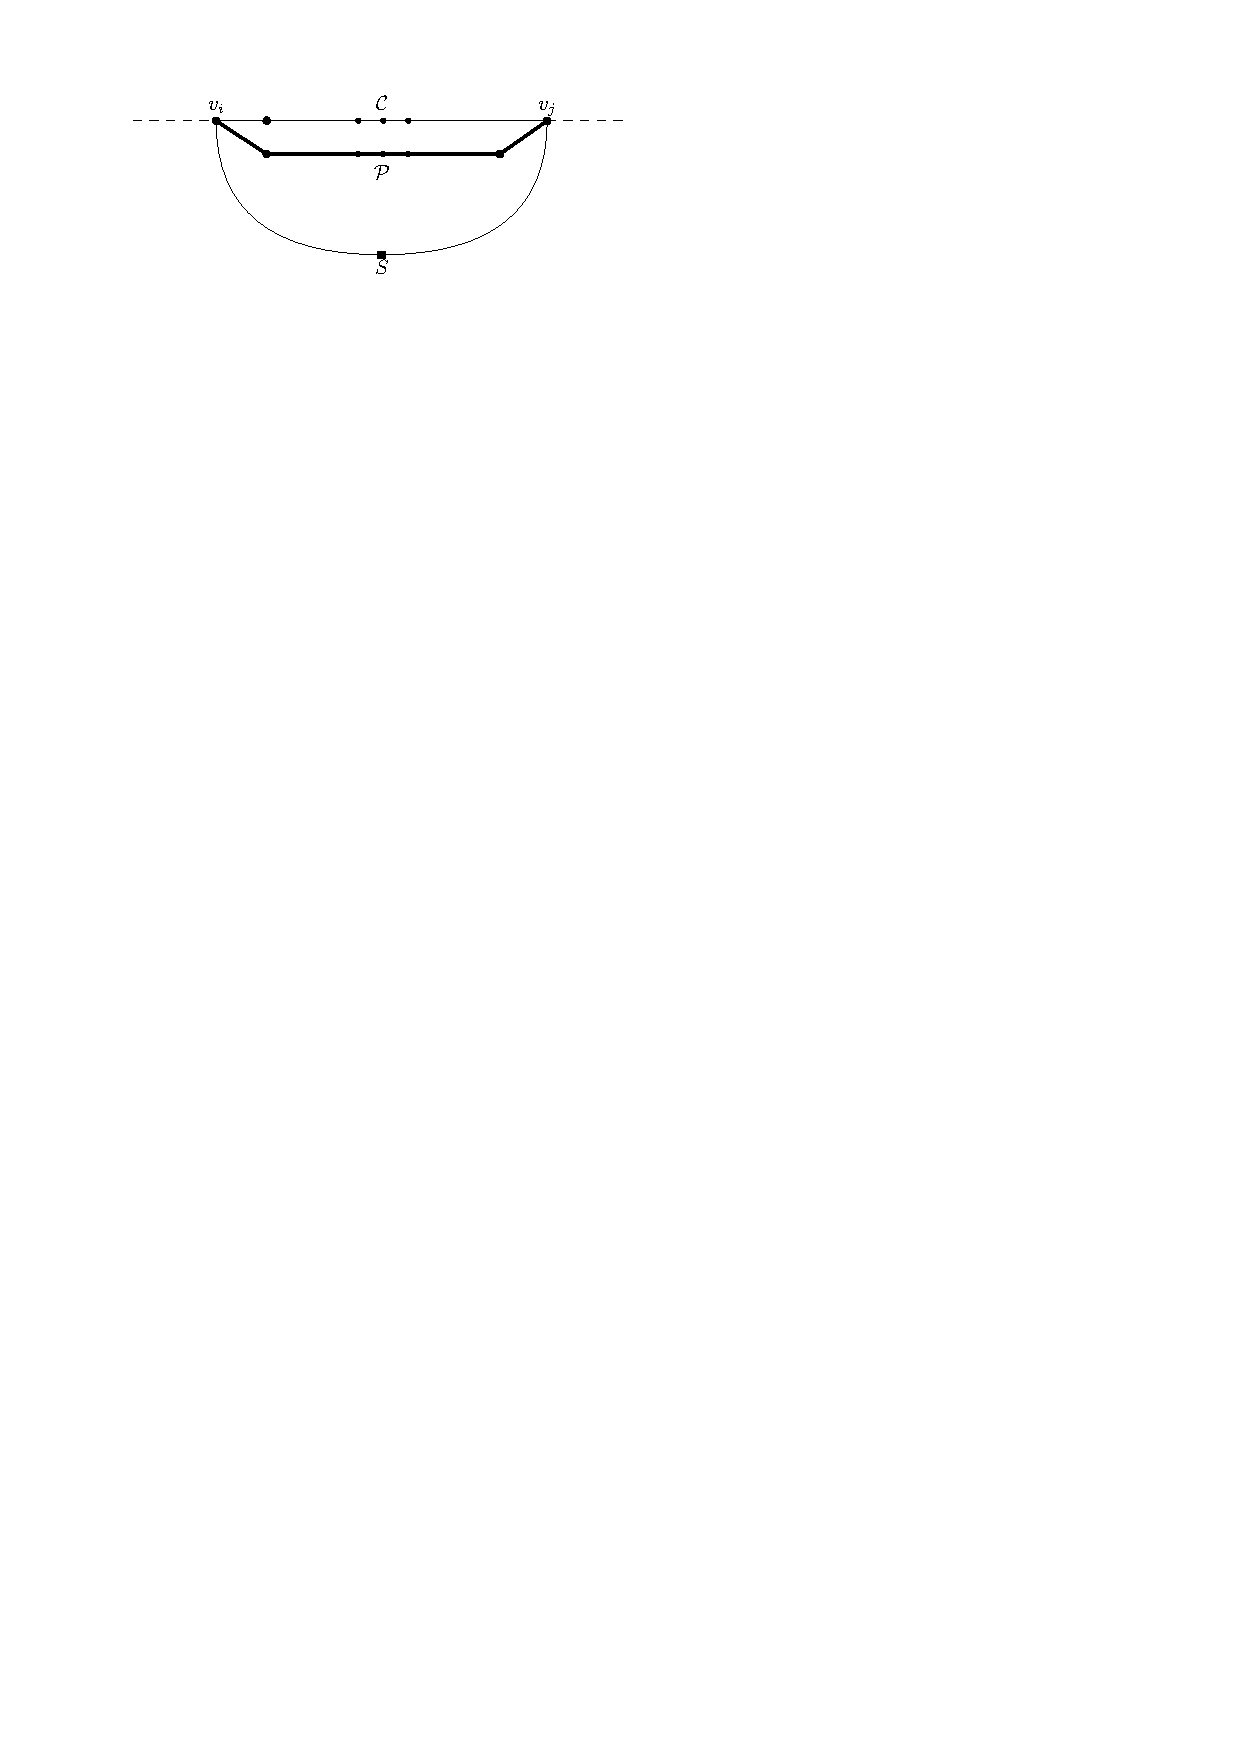
\includegraphics[scale=1]{unifiedAlgo/img/sweep/noIrregularity}
    \caption{Updating path when $P$ contains no irregularity.}
    \label{fig:sweep:noIrregularity}
  \end{figure}

\subsubsection{Evade chords and separating 2-chords}
  The candidate path $P$ we found can have two structures we want to avoid
  namely
  \begin{enumerate}
    \itemsep=-4pt
    \item Chords
    \item Separating 2-chords
  \end{enumerate}

  By \emph{irregularities} we will mean these two classes of structures together.
  All irregularities are on the right of the candidate path due to Lemma \ref{lm:right:neighbourwalkChordFree} (no chords on the left) and Lemma \ref{lm:right:neighbourwalkNoInteriorVertex} (no separating 2-chords on the left).

  Before we can show how to evade these structures we first introduce more notation. We orient $P$ from $v_i$ (the vertex closest to $\pW$)to $v_j$ (the vertex closest to $\pE$) and denote its vertices by $p_1 \ldots p_k$.
  The \emph{index} of a vertex $p_i \in P$ is its position in the path, that is, the index of $p_i$ is $i$.
  The \emph{start index} of a irregularity $I$ is the index of the first vertex in $P$ that is also in $I$. Similarly, the \emph{end index} is the index of the last vertex in $P$ that is also in $I$.
  The \emph{range} of an irregularity will be given by its start and end index. Depending on what irregularities we find on the candidate path $P$ we will update the sweepcycle with a \emph{update path} $P'$. This update is described in Section \ref{sss:sweep:update}.

  While describing the steps we will also show that the following two lemmas (Lemmas \ref{lm:sweep:augNoIregularity} and \ref{lm:sweep:noConnectingIregularity}) hold for every case.

  \begin{lemma}
    The updating paths have no chords or separating $2$-chords
    \label{lm:sweep:augNoIregularity}
  \end{lemma}

  \begin{lemma}
    \label{lm:sweep:noConnectingIregularity}
    There are no chords or separating $2$-chords not containing $\pS$ with one endpoint on the old sweepcycle and the other endpoint on the updating path.
  \end{lemma}

  \mypar{We have no irregularity}
    When there are no irregularities we update the sweepcycle with the entire candidate path $P$.
    In this case the update path $P'$ is equal to $P$.

    $P'$ has no irregularity by the definition of this case. Moreover, irrefuglaities with one ednopint on $P'$ and one endpoint on $\C$. Since $v_i$ and $v_j$ are both adjacent to $\pS$ we can not have any chords. And any $2$-chords must have $\pS$ as middle vertex.

  \mypar{We have any chord}
    Note that we can not have any polebound chords on the exterior vertices of the candidate path $P$ since any such chord would violate Invariant \ref{i:uni:no2Chords} of $\C$ as can been seen in Figure \ref{fig:sweep:noChordOnExteriorVertex}.

    \begin{figure}[h]
      \centering
      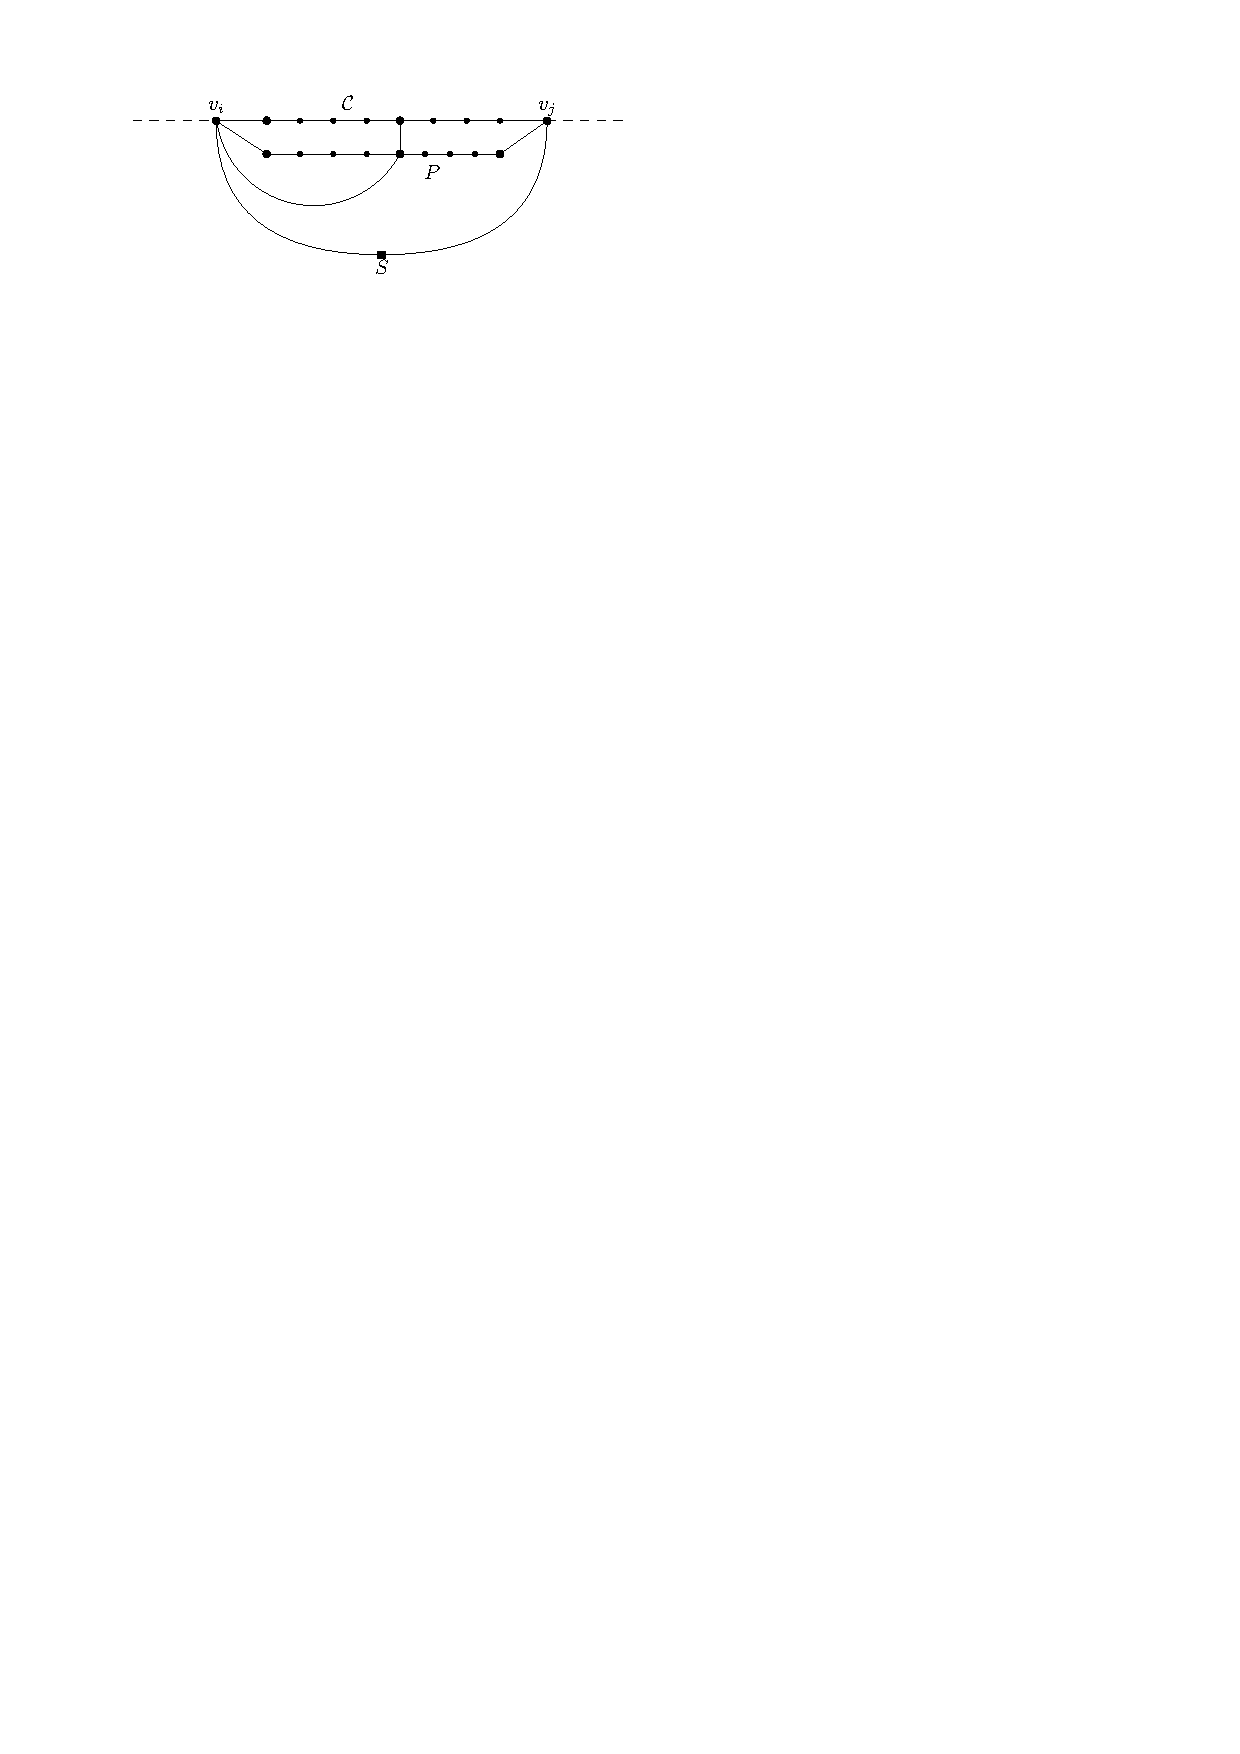
\includegraphics[scale=1]{unifiedAlgo/img/sweep/noChordOnExtriorVertex.pdf}
      \caption{Hypothetical situation where $P$ would have a chord on an exterior vertex.}
      \label{fig:sweep:noChordOnExteriorVertex}
    \end{figure}

    We identify the chords by their ranges. Of the chords with the smallest end index $j$ we will consider the one with the largest start index $i$. We denote this chord by $C$. Note that this chord can not contain any other chords since they would have either a large start index or a smaller end index.
    The way in which we find $C$ is illustrated in Figure \ref{fig:sweep:chordsOnCandidatePath}.

    \begin{figure}[b]
      \centering
      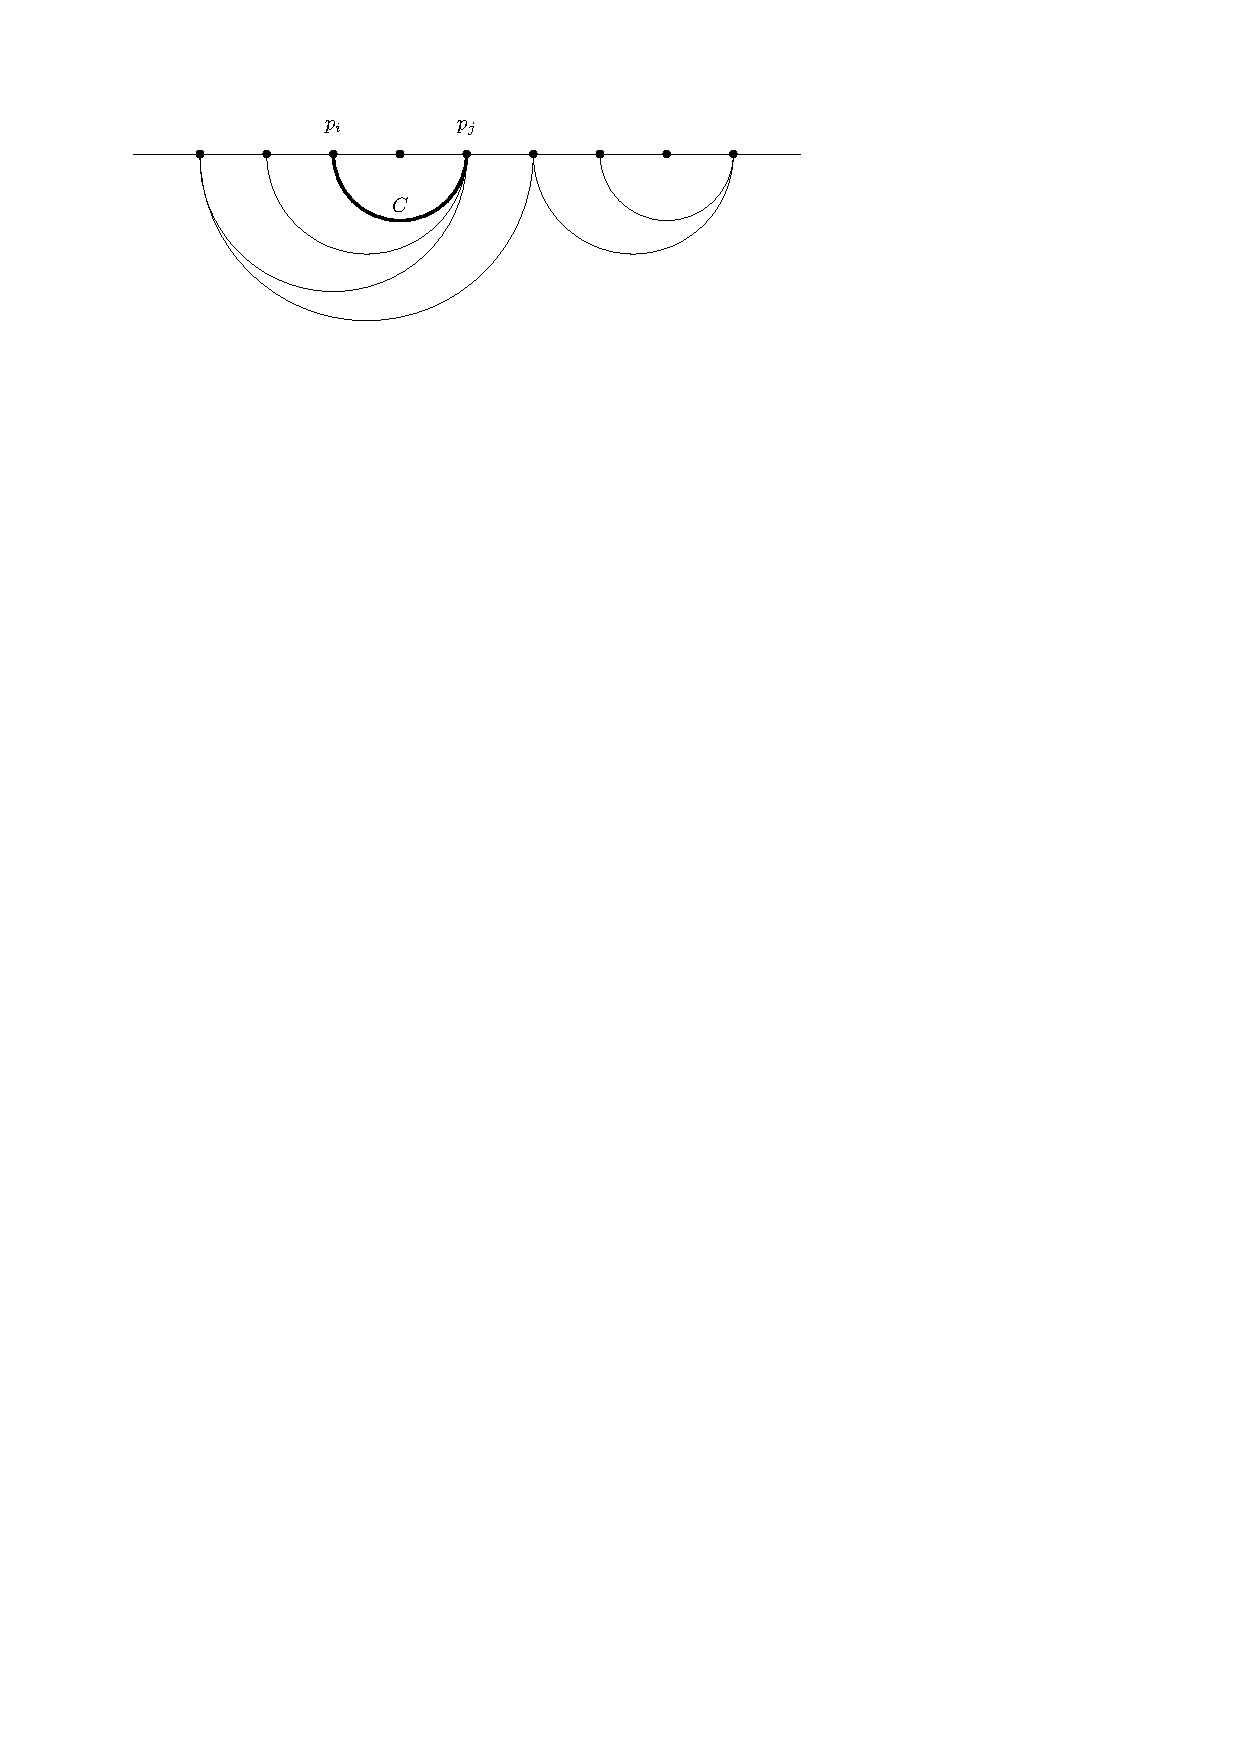
\includegraphics[scale=1]{unifiedalgo/img/sweep/chordsOnCandidatePath}
      \caption{Finding the chord $C$.}
      \label{fig:sweep:chordsOnCandidatePath}
    \end{figure}

    What we do now depends on whether a 2-chord shows up in the interior of the chord pasted to the candidate path $P|_{i, j} \oplus \rev{{C}}$.

    \emph{No separating 2-chord.}
    If there is no separating 2-chord in the interior of $P|_{i, j} \oplus \rev{{C}}$ we do the following. Let $v_k$ be the shared neighbor on $\C$ of $p_{i}$ and $p_{i +1}$ and $v_l$ the shared neighbor on $\C$ of $p_{j -1}$ and $p_{j}$. Then the updating path is the right neighbor path of $\cpath|_{v_k, v_l}$. See Figure \ref{fig:sweep:chordUpdate}.

    $P'$ is entirely inside a chord containing no more chords and thus can't contain a chord. Moreover, there are no separating $2$-chords on $P$ so $P'$ can not have separating $2$-chords. Any chord or separating $2$-chord with one endpoint in $P'$ and one in $\C$ will have to cross $v_k p_i p_j v_l$ so we can not have a chord. Any 2-chord has to have $p_i$ or $p_j$ as middle vertex. But with this restriction the 2-chord can not be separating.

    \begin{figure}[h]
      \centering
      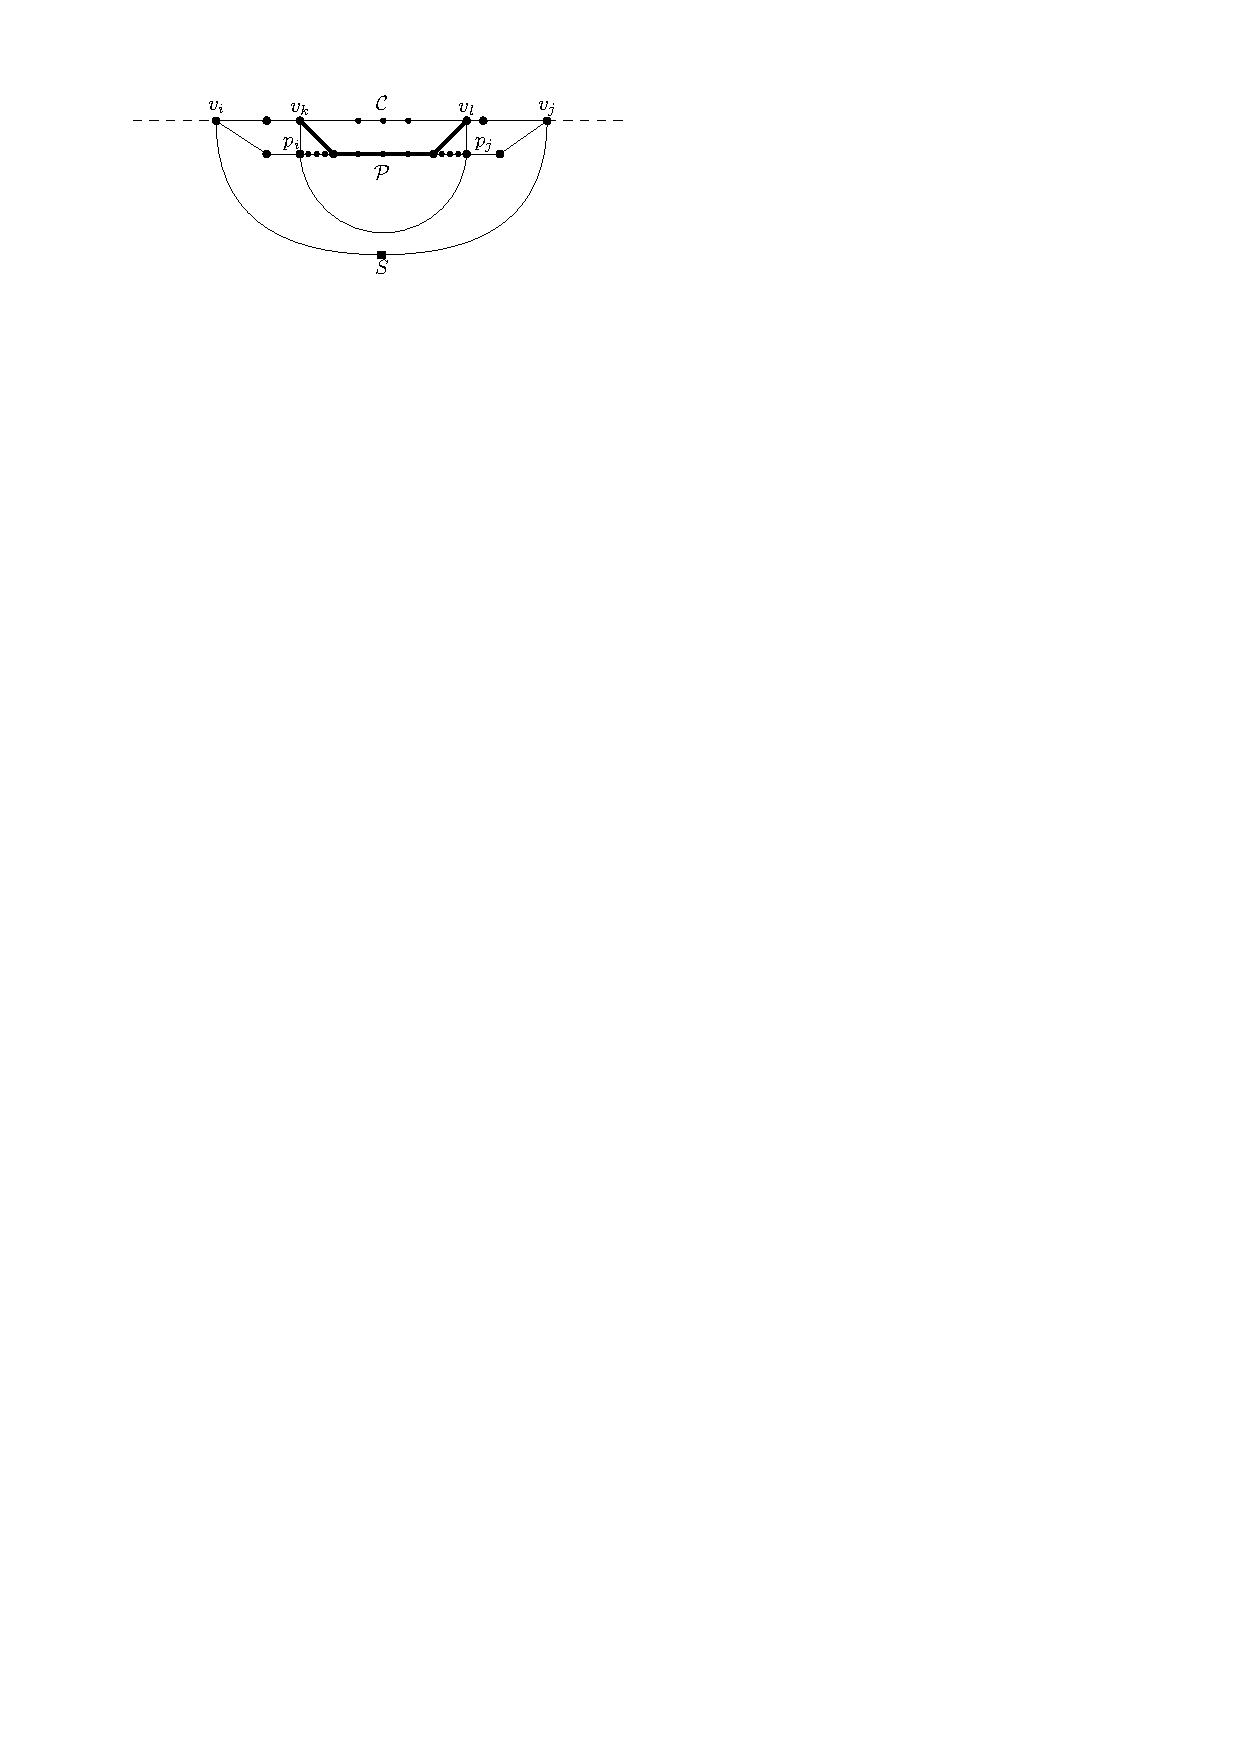
\includegraphics[scale=1]{unifiedAlgo/img/sweep/chordUpdate}
      \caption{Updating path when $P$ has a chord not containing a separating 2-chord.}
      \label{fig:sweep:chordUpdate}
    \end{figure}

    \emph{At least one separating 2-chord.}
      Let $j'$ be end index of the separating 2-chord with the lowest end index in the interior of $P|_{i, j} \oplus \rev{{C}}$. And let $v_k$ be the shared neighbor on the sweepcycle of $p_{i_1}$ $p_{i_1 +1}$ and $v_l$ the shared neighbor on the sweepcycle  of $p_{j' -1}$ and $p_{j'}$.
      Then the updating path $P'$ is the right neighbor path of $\cpath|_{v_k, v_l}$. See Figure \ref{fig:sweep:2chordInChordUpdate}.

      $P'$ is entirely inside a chord containing no more chords and thus can't contain a chord. Moreover, all separating $2$-chords are evaded since we evaded the ending of the first one ending.  In the same manner as in the above case we can not expect any chord or separating $2$-chord with one endpoint in $P'$ and one in $\C$ any chord or separating 2-chord to connect outside the containing chord.
      Suppose that we have a separating $2$-chord then that would have been a chord of the candidate path. This is in contradiction with the fact that the outer chord contained no more chords.
      Suppose that we have a chord not connecting to the second-to-last vertex of the updating path. This chord would violate Invariant \ref{i:uni:no2Chords} of the old sweepcycle. Furthermore the second-to-last vertex of the updating path has no chords since it would break $v_l p_j x p_u$. (see Figure \ref{fig:sweep:2chordInChordUpdate}).

      \begin{figure}[h]
        \centering
        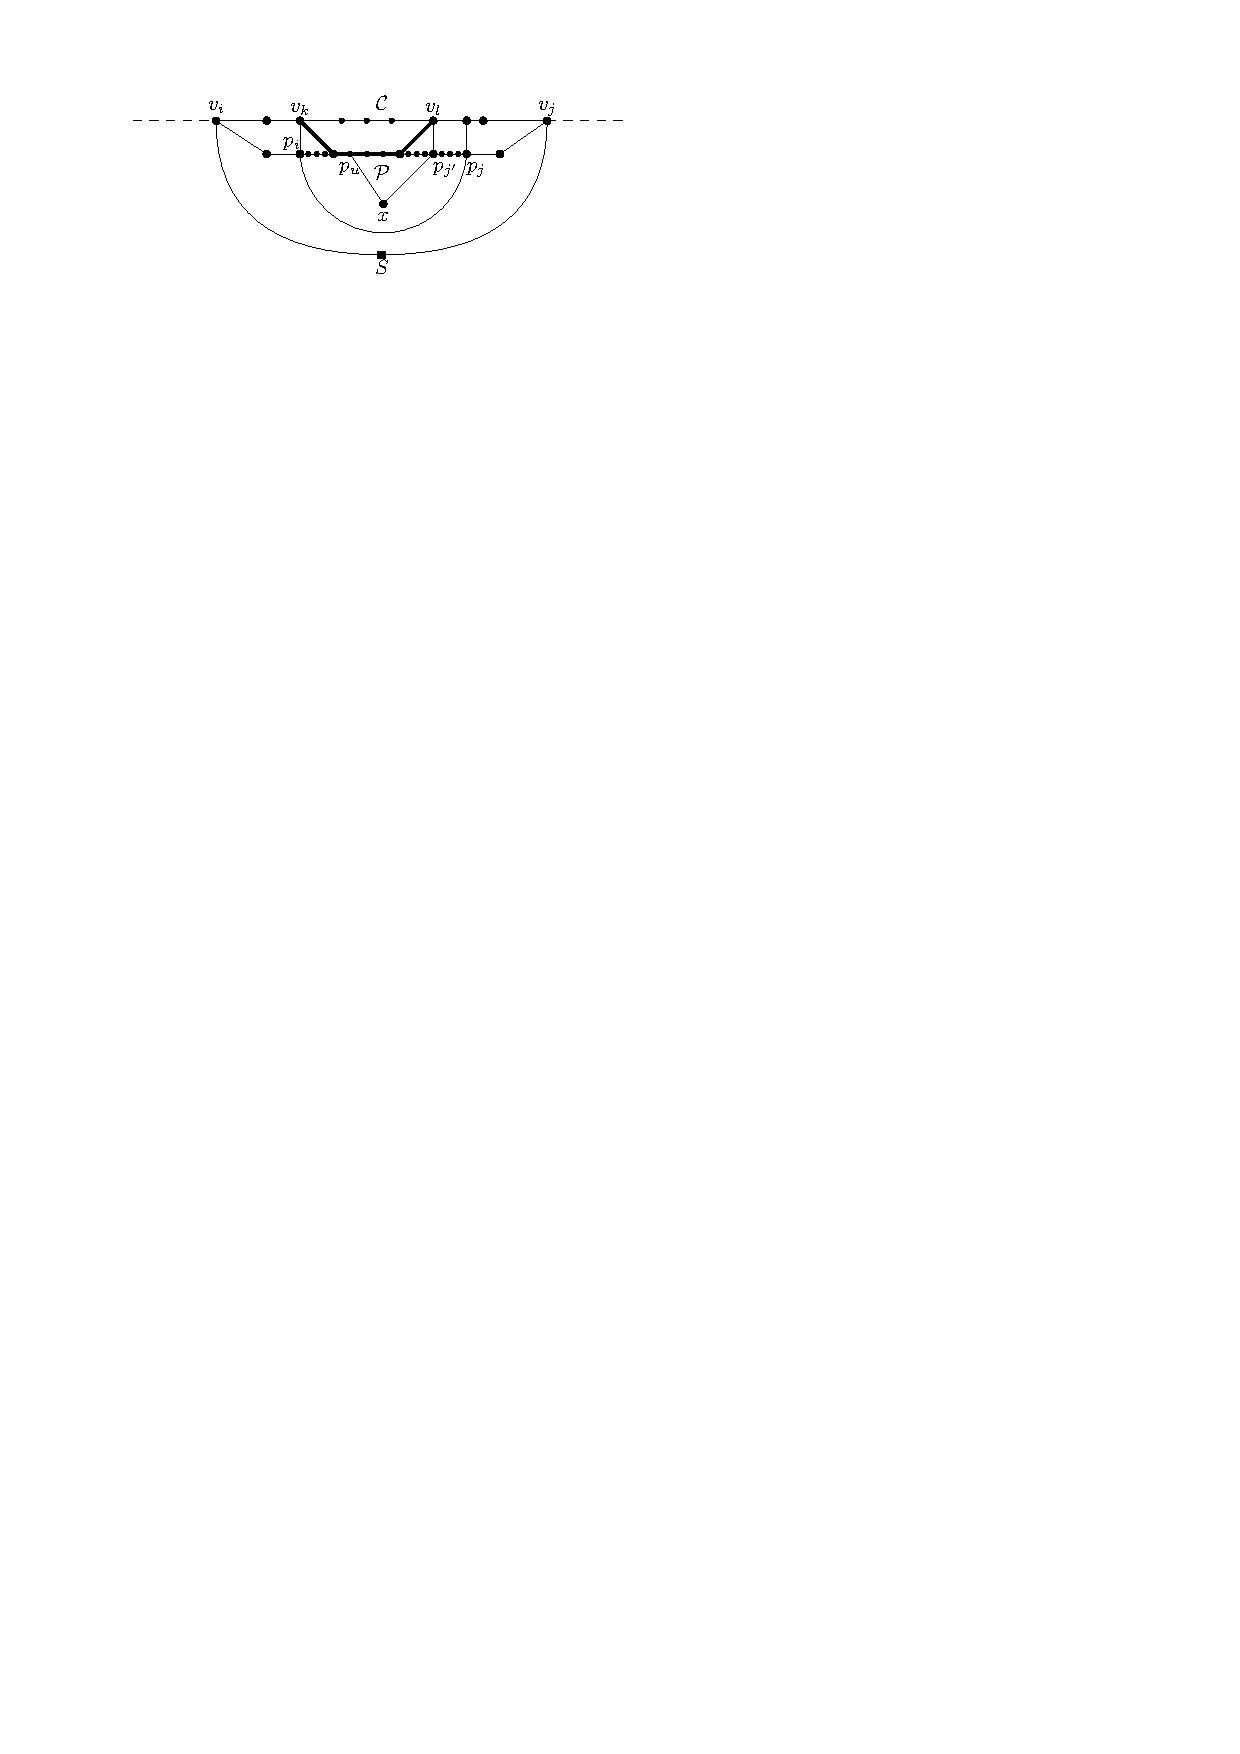
\includegraphics[scale=1]{unifiedAlgo/img/sweep/2chordInChordUpdate}
        \caption{Updating path when $P$ has a chord containing at least one separating 2-chord.}
        \label{fig:sweep:2chordInChordUpdate}
      \end{figure}

  \mypar{Only separating 2-chords}
    In this case the candidate path $P$ has no chords since otherwise we would be in the above case.
    \emph{Any separating 2-chords with $v_j$ as end vertex.}
      We find the smallest separating 2-chord (i.e. with the highest start index). Say this separating $2$-chord has start index $i$.
      Let $v_k$ be the shared neighbor on the sweepcycle of $p_{i}$ and $p_{i +1}$. The updating path is the right neighbor path of $\cpath|_{v_k, v_j}$. See Figure \ref{fig:sweep:pEBound}.

      $P'$ has no chords. Moreover, $P'$ starts inside the smallest separating $2$-chord hence it has no $2$-chords.

      We can not have any chords with one endpoint in $P'$ and one in $\C$  since these would have to break $\pE x p_i v_k$. Any $2$-chords with one endpoint in $P'$ and one in $\C$ would have $x$ or $p_i$ as middle vertex. However the first yields a $2$-chord of the candidate path with a higher start range, this is a contradiction. And the second can not yield an separating $2$-chord.

    \begin{figure}[h]
      \centering
      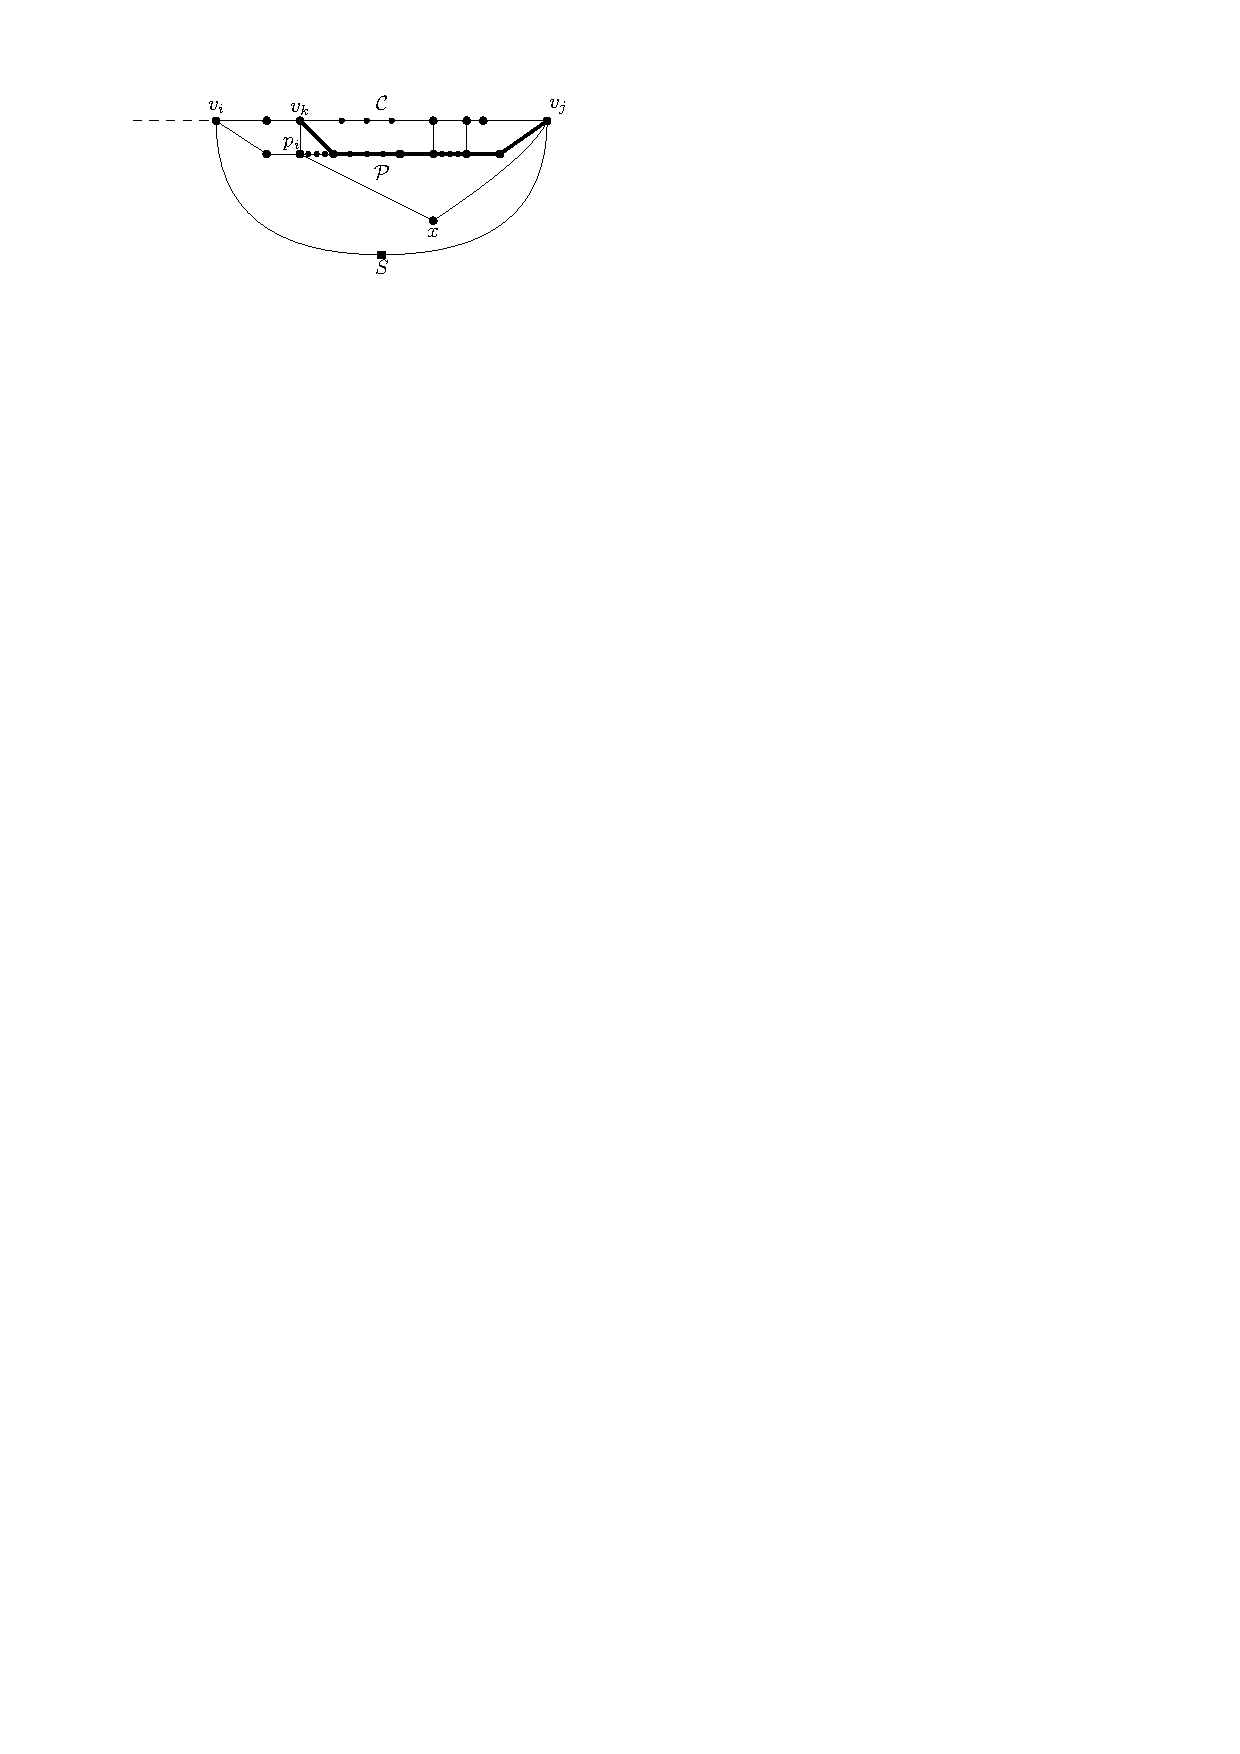
\includegraphics[scale=1]{unifiedAlgo/img/sweep/pEBound}
      \caption{Updating path when $P$ has a separating 2-chord with $v_j$ as end vertex.}
      \label{fig:sweep:pEBound}
    \end{figure}

    \emph{Only other separating 2-chords}
      Find the $2$-chord with the lowest end index, say that this is $j$.
      Let $v_l$ be the shared neighbor on the sweepcycle of $p_{j}$ and $p_{j-1}$.
      The updating path is the right neighbor path of $\cpath|_{v_i, v_l}$. See Figure \ref{fig:sweep:free2chord}.

      Any updating path stops before the end of a separating 2-chord and furthermore conatins no chords since $P$ already didn't.

      Any chord or $2$-chord with one vertex in the updating path and the other on the old sweepcycle must end to the right of the updating path since the updating path starts at $\pW$.
      Suppose that we have a separating $2$-chord then that would have been a chord of the candidate path. This is in contradiction with the assumption that the candidate path had no chords.
      Suppose that we have a chord not connecting to the second-to-last vertex of the updating path. This chord would violate Invariant \ref{i:uni:no2Chords} of the old sweepcycle. Furthermore the second-to-last vertex of the updating path has no chords since it would break $v_l p_j x p_u$. (see Figure \ref{fig:sweep:free2chord}).

    \begin{figure}[b]
      \centering
      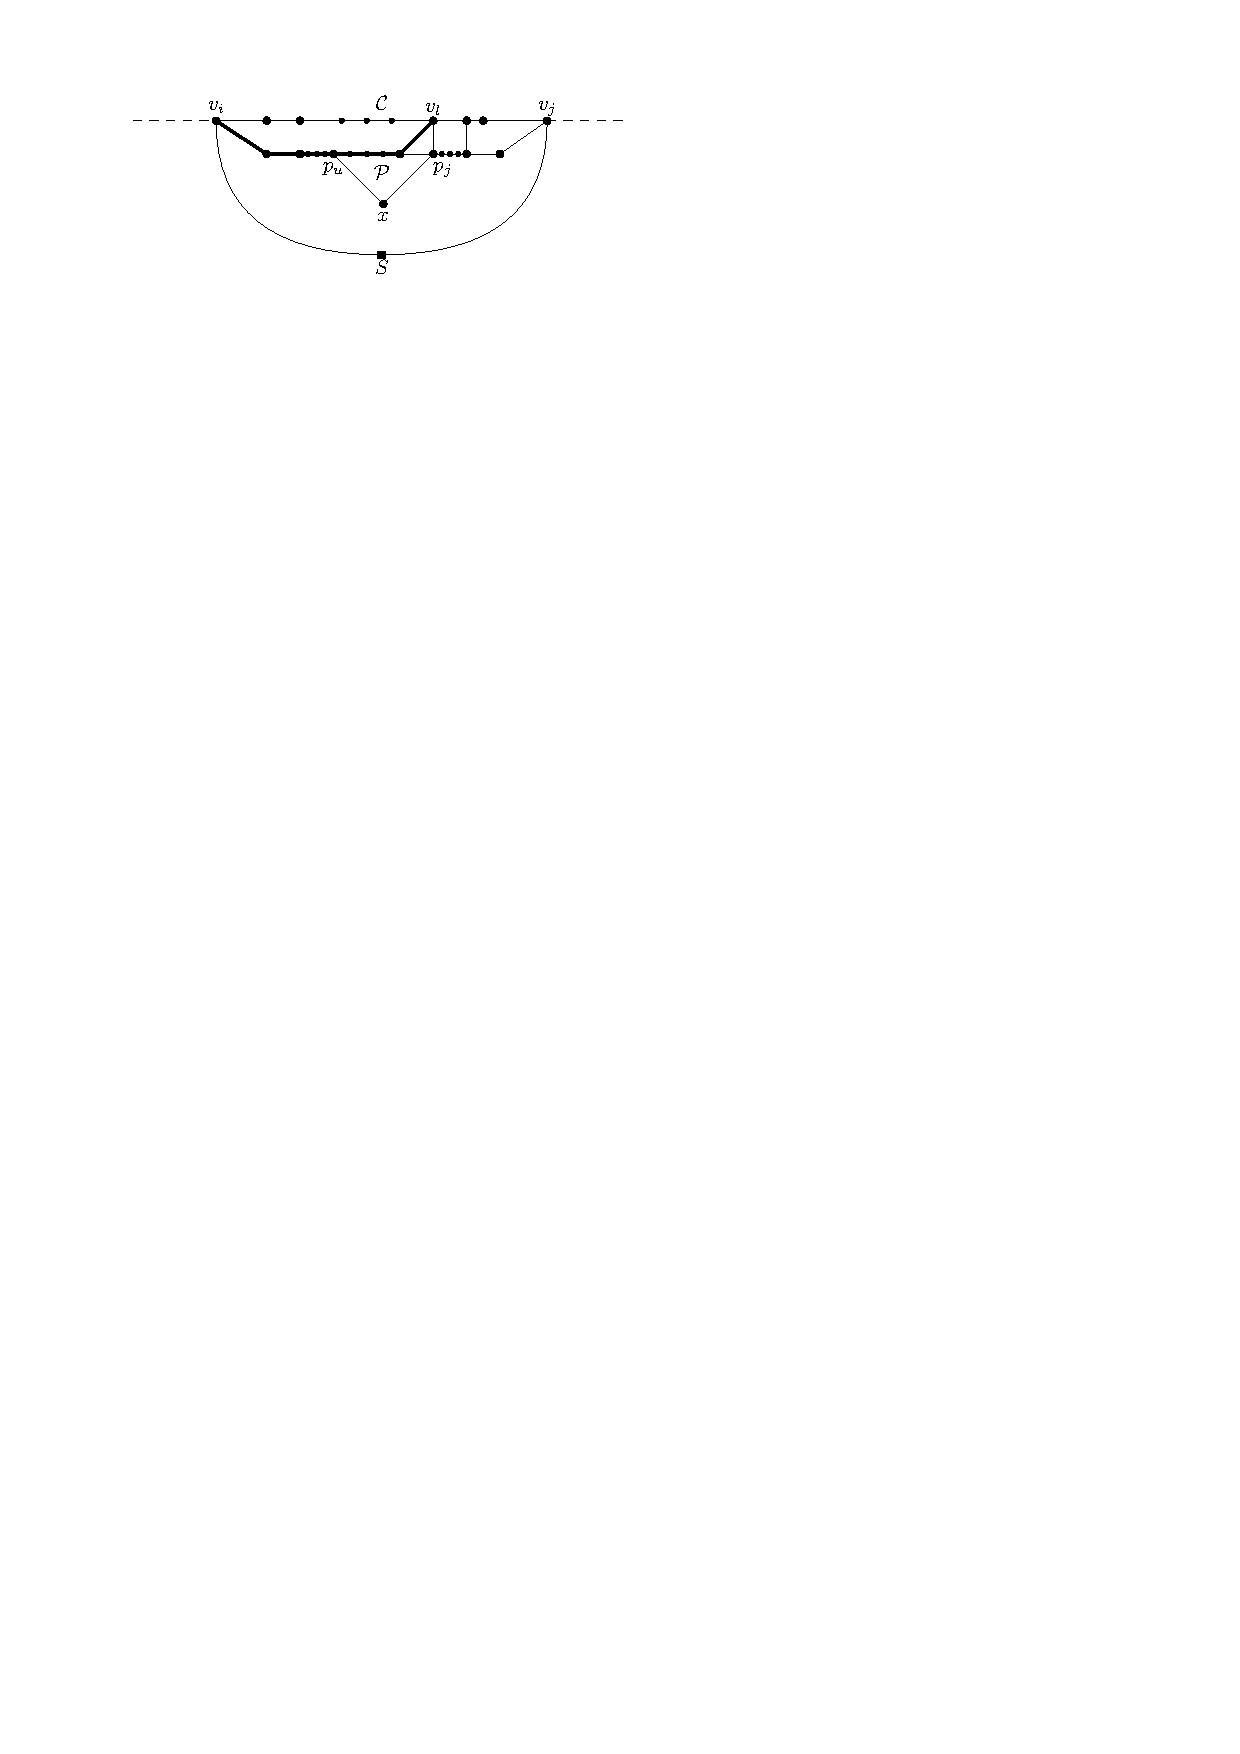
\includegraphics[scale=1]{unifiedAlgo/img/sweep/free2chord}
      \caption{Updating path when $P$ has separating 2-chords none of which have $v_j$ as end vertex.}
      \label{fig:sweep:free2chord}
    \end{figure}

\subsubsection{Updating}
  \label{sss:sweep:update}
  Once we found the updating path $P'$ we can update the sweepcycle with this path.
  We describe how to do this and we also show that the update maintains the sweepcycle invariants (Lemma \ref{lm:sweep:updateMaintainsInvariants}).
  To update we color all interior edge of $\cpath|_{P'} \oplus \rev{P'}$ red and orient them towards $\cpath|_{P'}$.
  We also color all edges of $\cpath|_{P'}$  blue and orient them from lower to higher induces.
  We then update the sweepcycle to $\C'$ by replacing $\cpath|_{v_i,v_j}$ by $P'$ in $\C$.
  An example of the whole update for a updating path $P'$ can be seen in Figure \ref{fig:sweep:update}.

  \begin{figure}
      \centering
      \begin{subfigure}[b]{0.45 \textwidth}
          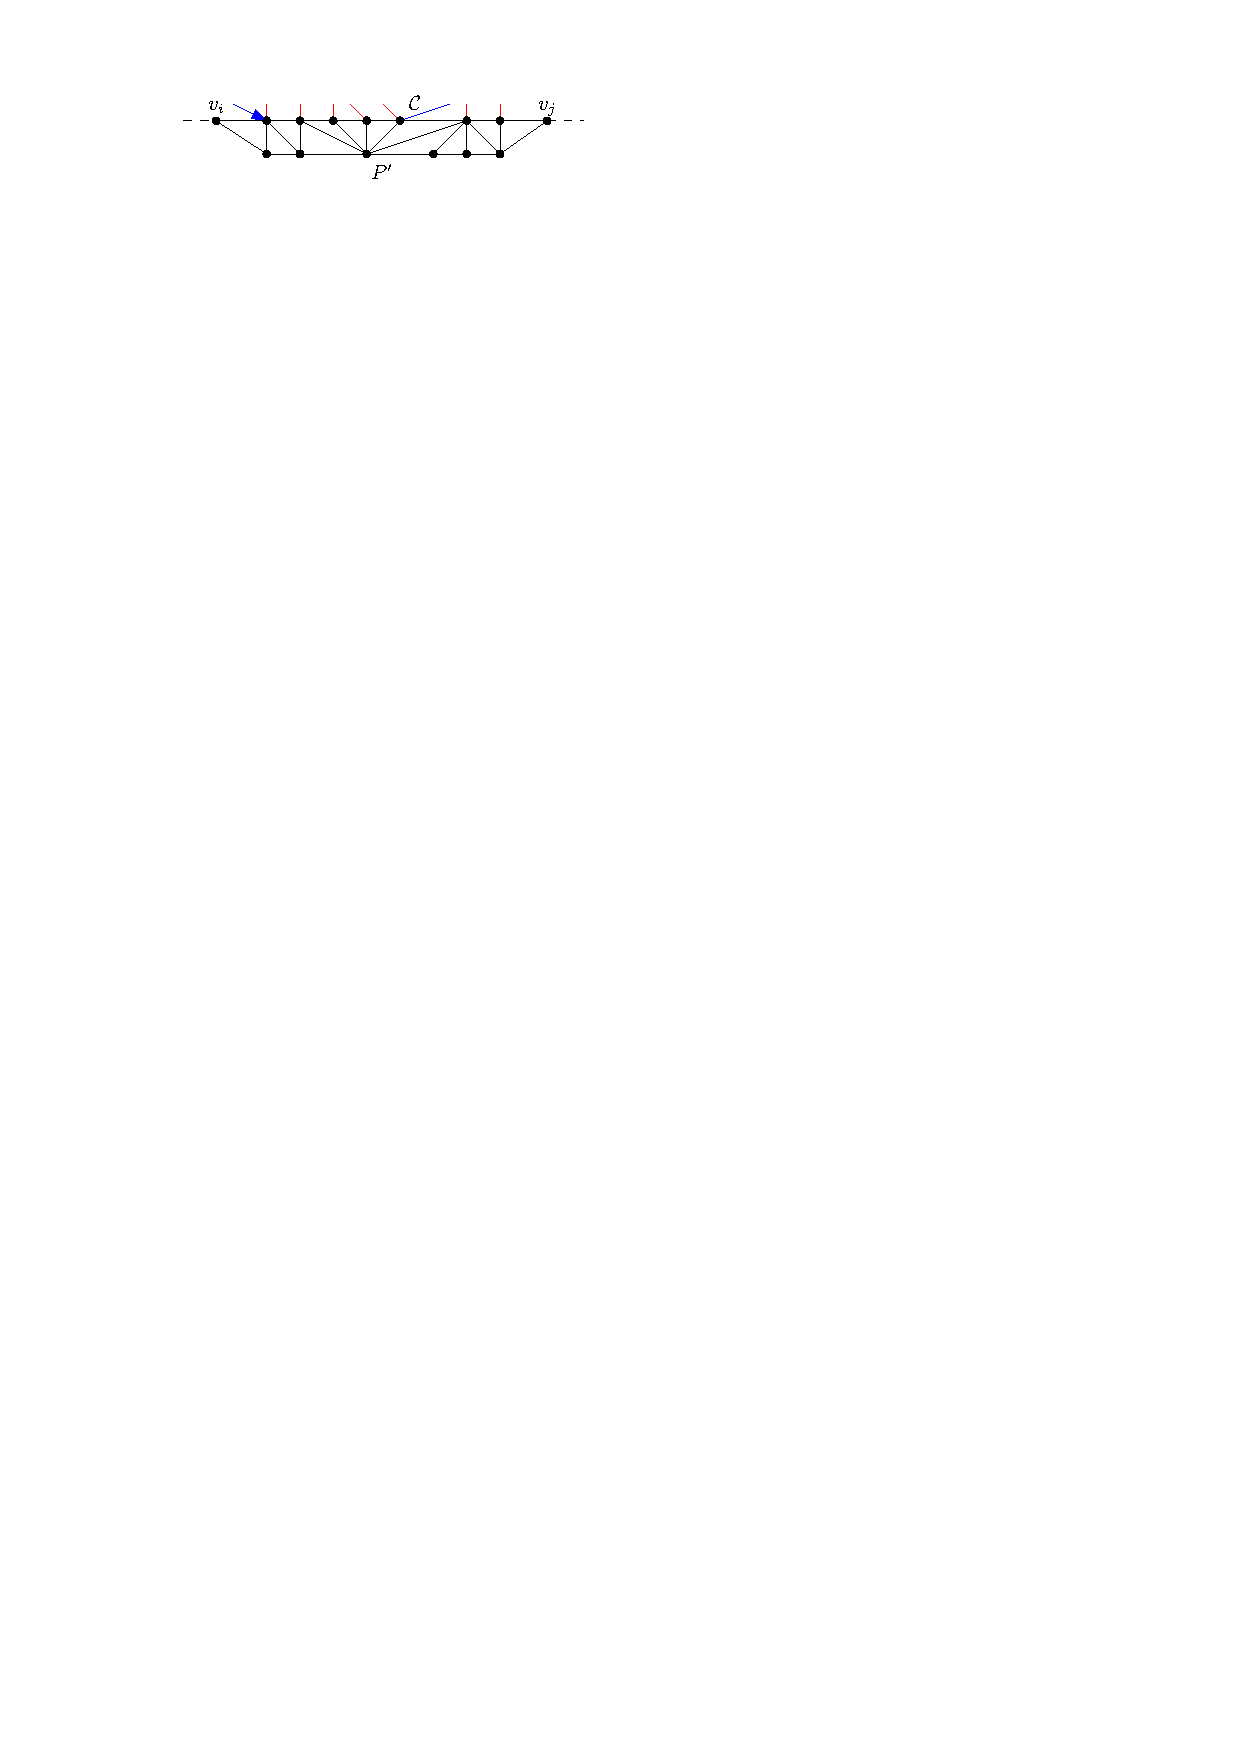
\includegraphics[width = \textwidth]{unifiedAlgo/img/sweep/updateBefore.pdf}
          \caption{Before.}
      \end{subfigure}
      ~
      \begin{subfigure}[b]{0.45 \textwidth}
          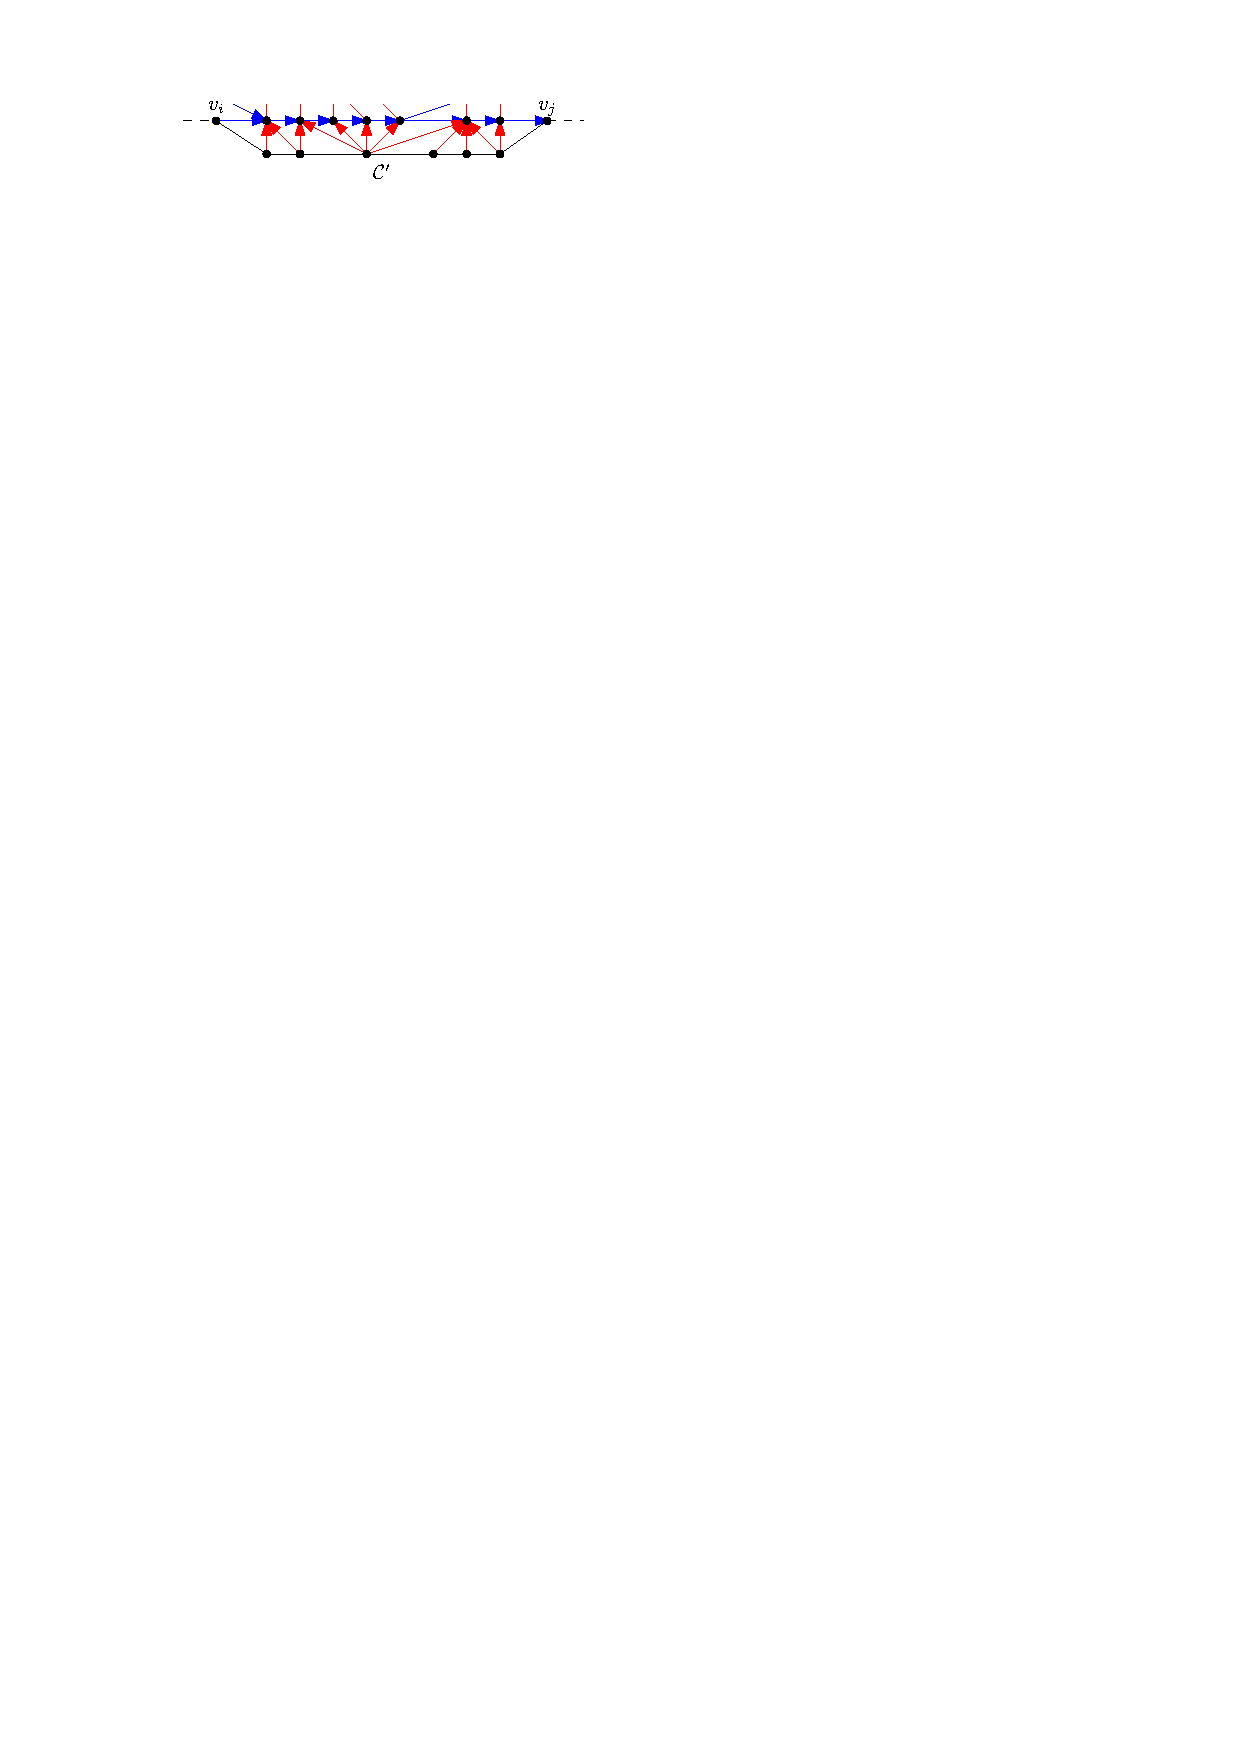
\includegraphics[width =\textwidth]{unifiedAlgo/img/sweep/updateAfter.pdf}
          \caption{After.}
      \end{subfigure}
      	\caption{The update.}
  \label{fig:sweep:update}
  \end{figure}


  \begin{lemma}
    \label{lm:sweep:updateMaintainsInvariants}
    All five updating path types maintain the sweepcycle invariants
  \end{lemma}
  \begin{proof}
    We will proof that the new sweepcycle $\C'$ obtained by updating $\C$ is again a valid sweepcycle. Invariant \ref{i:uni:SWandSE} remains trivially true. Invariant \ref{i:uni:intVertCond} hold due to the way we colored the edges around the new interior vertices as can be seen in Figure \ref{fig:sweep:update}.

    To see that Invariants \ref{i:uni:noChords} and \ref{i:uni:no2Chords} hold note that there can be no chords or $2$-chords with both endpoints in the overlap of the old and new sweepcycle $\C \cap \C'$ by the same Invariants \ref{i:uni:noChords} and \ref{i:uni:no2Chords}. Since the updating path itself also has no irregularities (Lemma \ref{lm:sweep:augNoIregularity}),
    we know any chord or separating $2$-chord $C$ has to have one vertex on $\P$ and one vertex on the unchanged part of old sweepcycle $\C \cap \C'$.
    However these potential chords can not exist by Lemma \ref{lm:sweep:noConnectingIregularity}.
    Hence $\C'$ is a valid new sweepcycle.
  \end{proof}

  If after the update the new sweepcycle $\C'$ has no interior vertices we terminate the algorithm as will be described in Section \ref{sss:terminating}. Otherwise we start the loop again by finding a new candidate path.

\subsubsection{Terminating}
  \label{sss:terminating}
  When the sweepcycle has no more interior vertices we can not update it anymore.
  However, at this point it is easy to color the remainder of the graph.
  All vertices in $\cpath$ must be adjacent to $\pS$ since $\pS \pW$ and $\pS \pE$ are part of $\C$ by Invariant \ref{i:uni:SWandSE}, $\cpath$ has no chords by Invariant \ref{i:uni:noChords} and $\C$ does not contain any interior vertices. Since all vertices are adjacent to $\pS$ all sweepcycle interior edges are adjacent to $\pS$.

  We color all interior edges of $\C$ red and orient them towards $\cpath$ and the edges in $\cpath$ are colored blue and oriented towards $\pE$. The termination step can be seen in Figure \ref{fig:sweep:terminate}. This last move completes the interior vertex condition for vertices in $\C \sm {\pW, \pS, \pE}$ and also correctly completes the exterior vertex condition.


  \begin{figure}[h]
    \centering
    \begin{subfigure}[b]{0.45 \textwidth}
        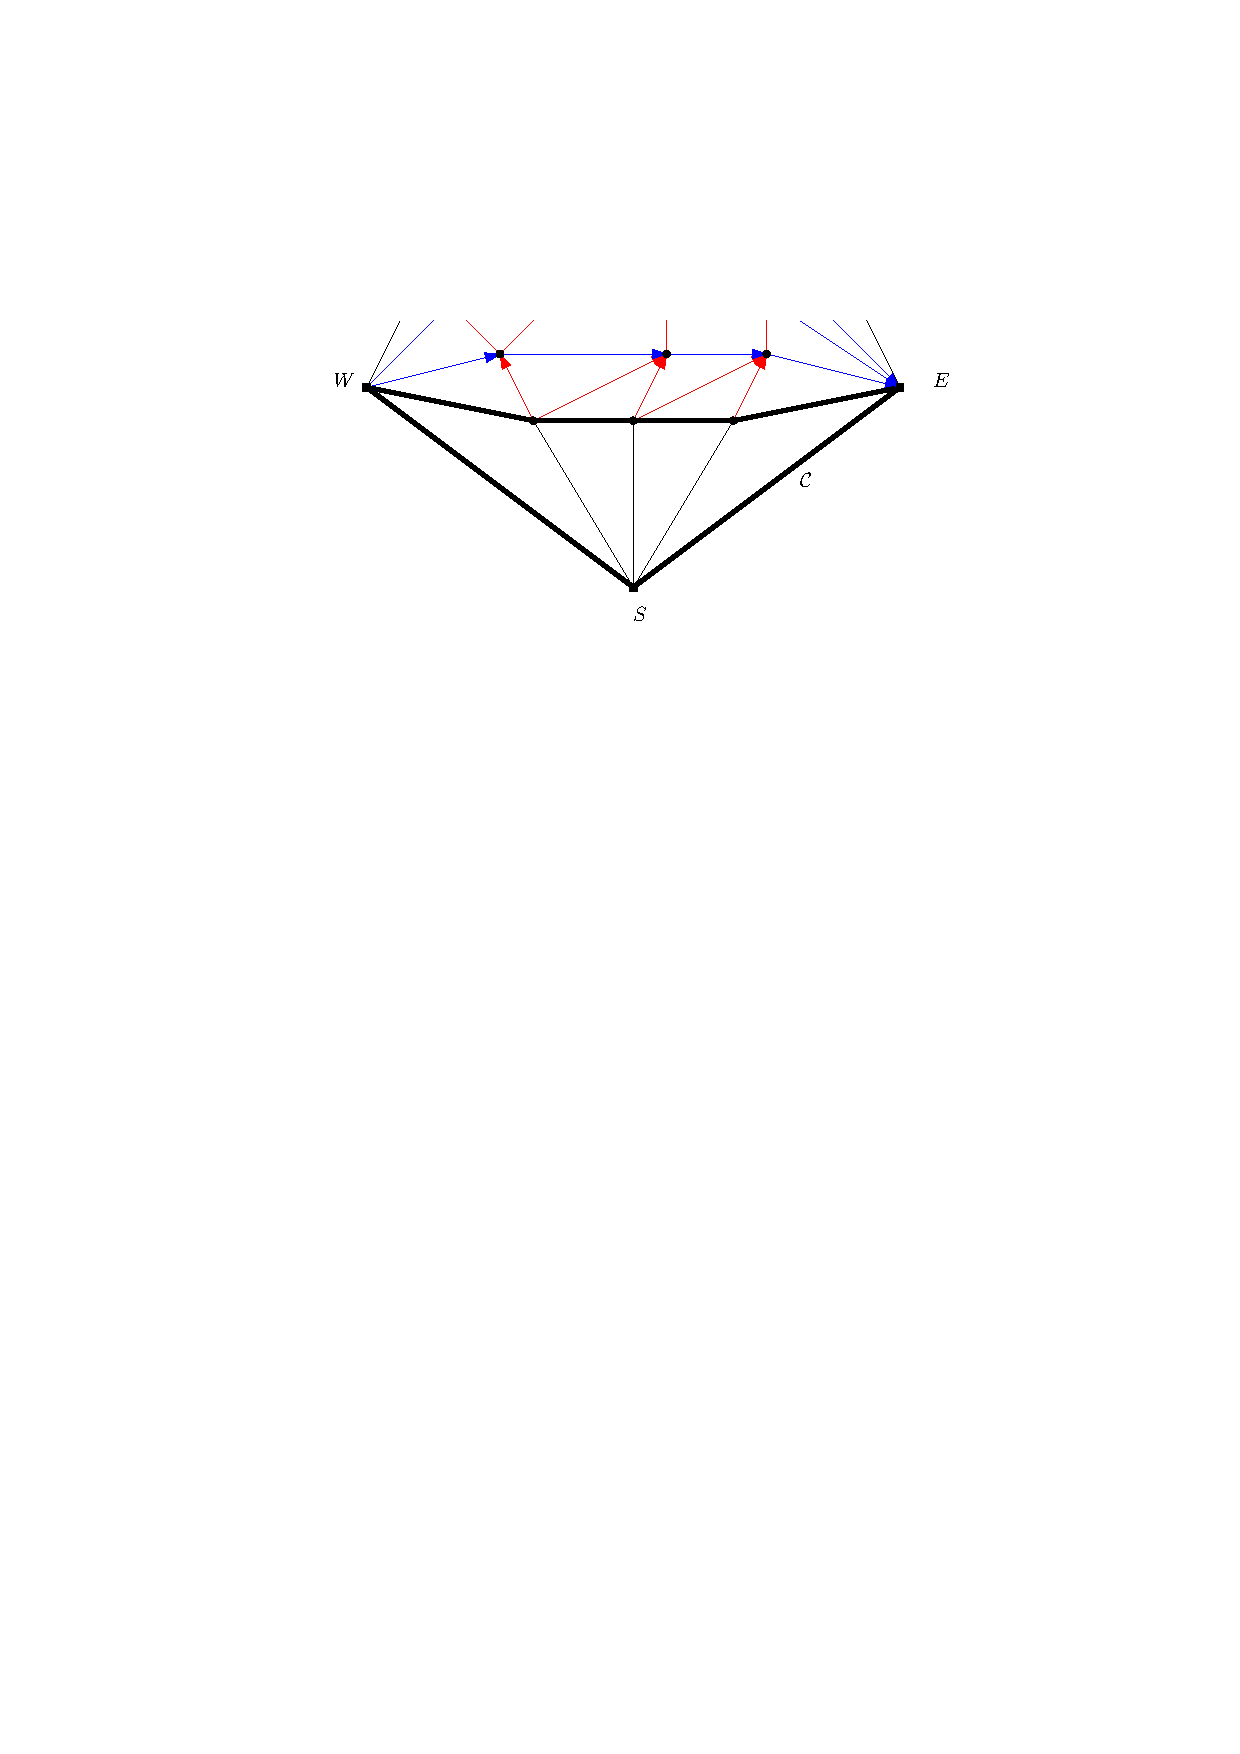
\includegraphics[width = \textwidth]{unifiedAlgo/img/sweep/terminateBefore.pdf}
        \caption{Before.}
    \end{subfigure}
    ~
    \begin{subfigure}[b]{0.45 \textwidth}
        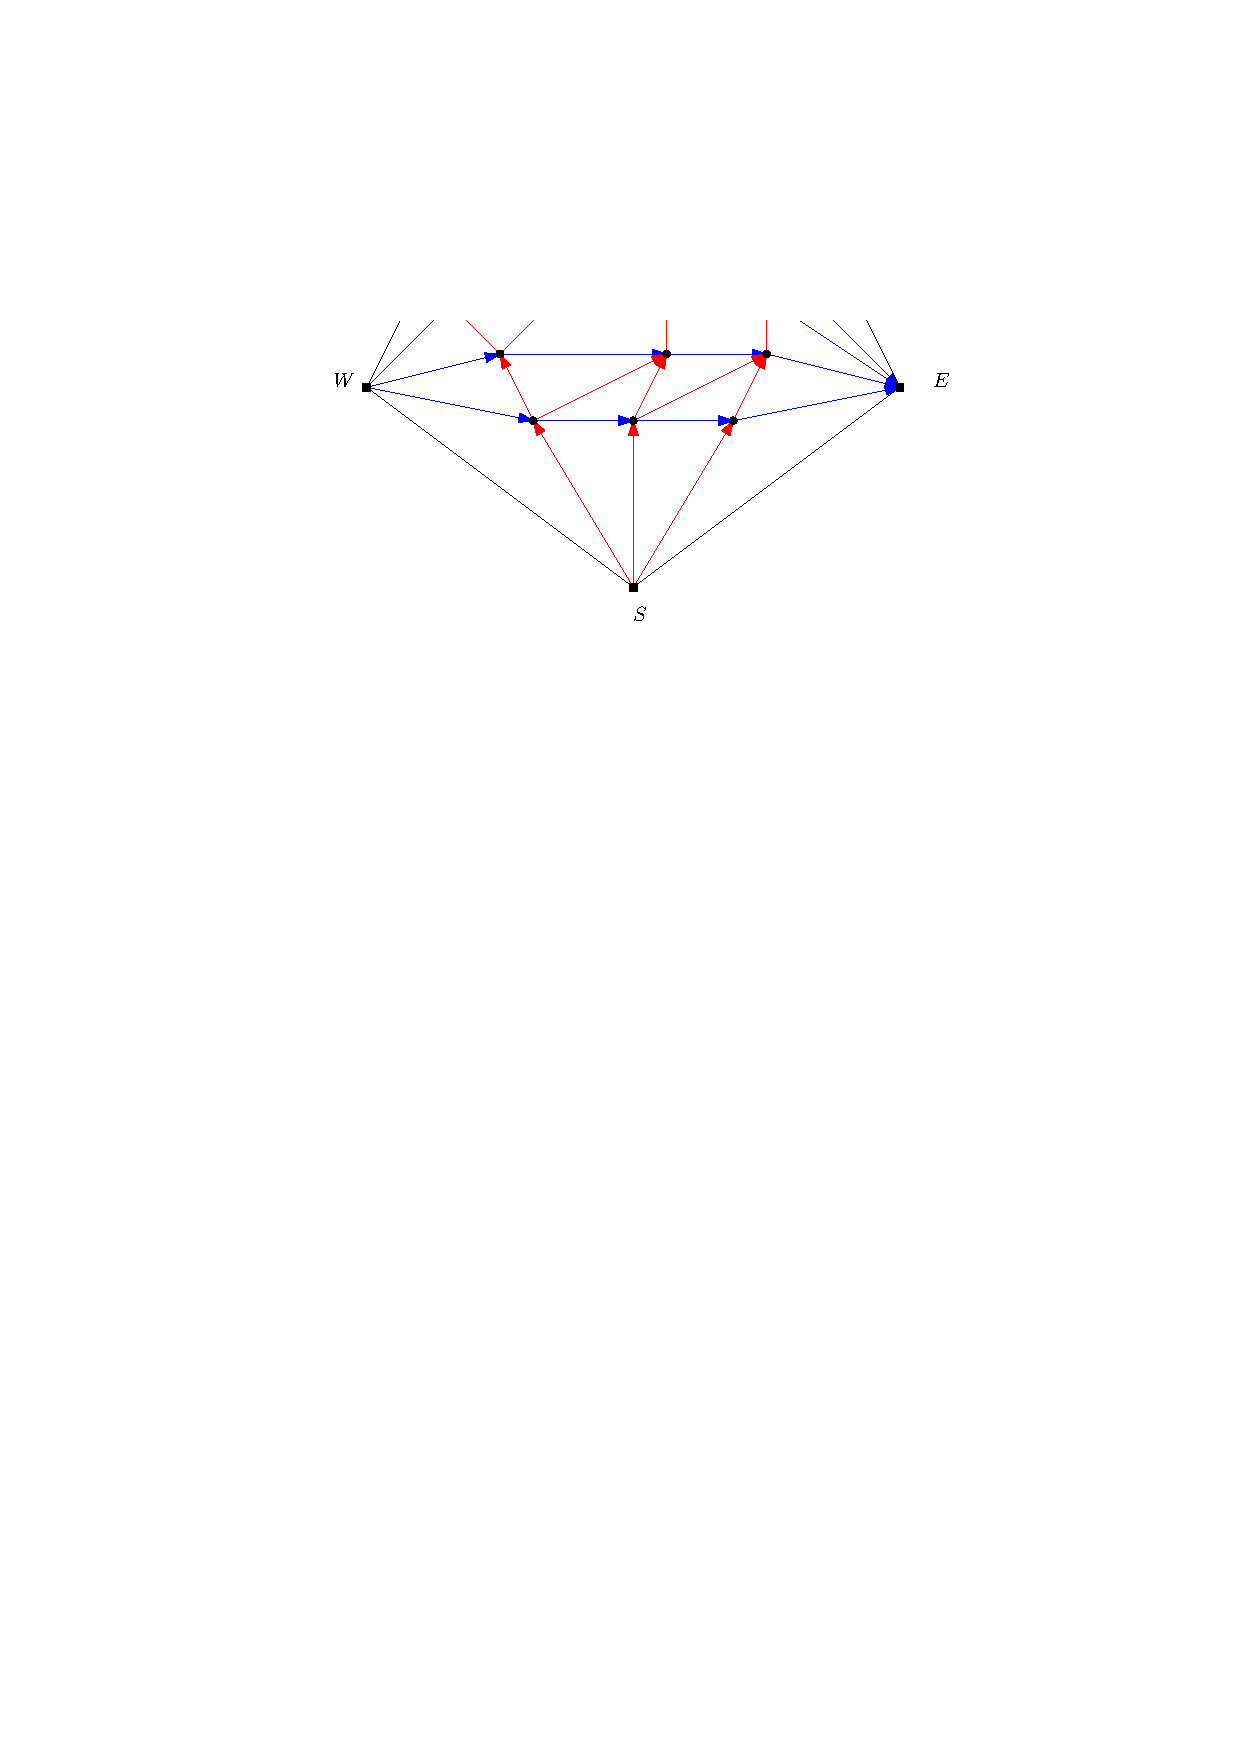
\includegraphics[width =\textwidth]{unifiedAlgo/img/sweep/terminateAfter.pdf}
        \caption{After.}
    \end{subfigure}
    \caption{The termination step.}
    \label{fig:sweep:terminate}
  \end{figure}

  \begin{lemma}
    \label{lm:sweep:REL}
    The resulting structure is a REL
  \end{lemma}

  \begin{proof}
    After running the whole algorithm the interior vertex condition holds for all vertices in the graph. Furthermore the poles are also colored correctly due to Invariant \ref{i:uni:SWandSE}.
  \end{proof}


  \mypar{Fans}
    There still is a very useful property of this regular edge labeling left to discuss (Lemma \ref{lm:sweep:NoTwoSplitsAboveEachOther}). Before we can state this property we first need to introduce fans.


    We want to better describe the interior of blue (or red) faces. Every interior edge of such face goes from one boundary path to the other (otherwise its start or end vertex would violate the interior vertex condition). We will describe the edges from the split to the merge vertex of $F$.

    Let $u_0 , u_1, \ldots u_n$ be the vertices of the top boundary path of $F$ and $v_0, v_1, \ldots, v_m$ the vertices of the bottom boundary path. That is $u_0=v_0$ is the split vertex and $u_n = v_m$ is the merge vertex. Since our graph is a triangulation $u_1v_1$ must be an edge. For the second edge in the face we have two options $u_1v_2$ or $u_2v_1$, otherwise this edge and the previous one would not form a triangle. This principle holds for every subsequent edge, we can either increase the index of the top boundary path or the index of the bottom boundary path. In other words, this face is a so-called \emph{triangle strip}.

    We call a maximal sequence of at least two edges increasing the index on the bottom boundary path (and thus keeping the index on the upper path fixed) a \emph{bottomfan} or simply \emph{B-fan} and a maximal sequence of at least two edges increasing the index on the top boundary path is called a \emph{topfan} or just \emph{T-fan}.
    The \emph{size} of such a fan is the number of edges contained in the sequence. By the definition of a fan it has size of at least $2$.
    We use \emph{fans} to refer to both these \emph{types} of fans (i.e. T- and B-fans).
    We call a fan of size $3$ or larger a \emph{large fan} and a fan of size $2$ a \emph{small fan}.

    In a strip we alternately encounter B- and T-fans. Since if we would have two adjacent fans of the same type we would just have a single larger fan of that type.
    In Figure \ref{fig:uni:fans} we see a strip consisting of subsequently a B-fan of size $3$, a T-fan of size 2, a B-fan of size $2$, a T-fan of size $6$, a B-fan of size $3$ and a T-fan of size $3$.



     We introduce some more terminology for fans: \emph{outer edges}, \emph{fan handles} and the \emph{rim} as can be seen in Figure \ref{fig:rect:fanTerms}. The \emph{fan handle} $v$ is the vertex shared by all edges in the fan. Let $H$ be the induced subgraph of vertices incident to the edges in the fan. $H$ contains no edges not belonging to $F$ since these would lead to separating 3-cycles. The \emph{rim} is the path given by $F\sm{v}$.
     \fxnote{Q is this definition of Rim more clear or still unclear?}
     The \emph{outer rim} are the two extreme edges of this path and the \emph{outer edges} are the edges between the fan handles and the extreme vertices of the \emph{rim}.

     A very similar discussion can be given for red faces. However then we will talk about \emph{right fans} and \emph{left fans} instead of bottom and top fans

     \begin{figure}[h]
       \centering
       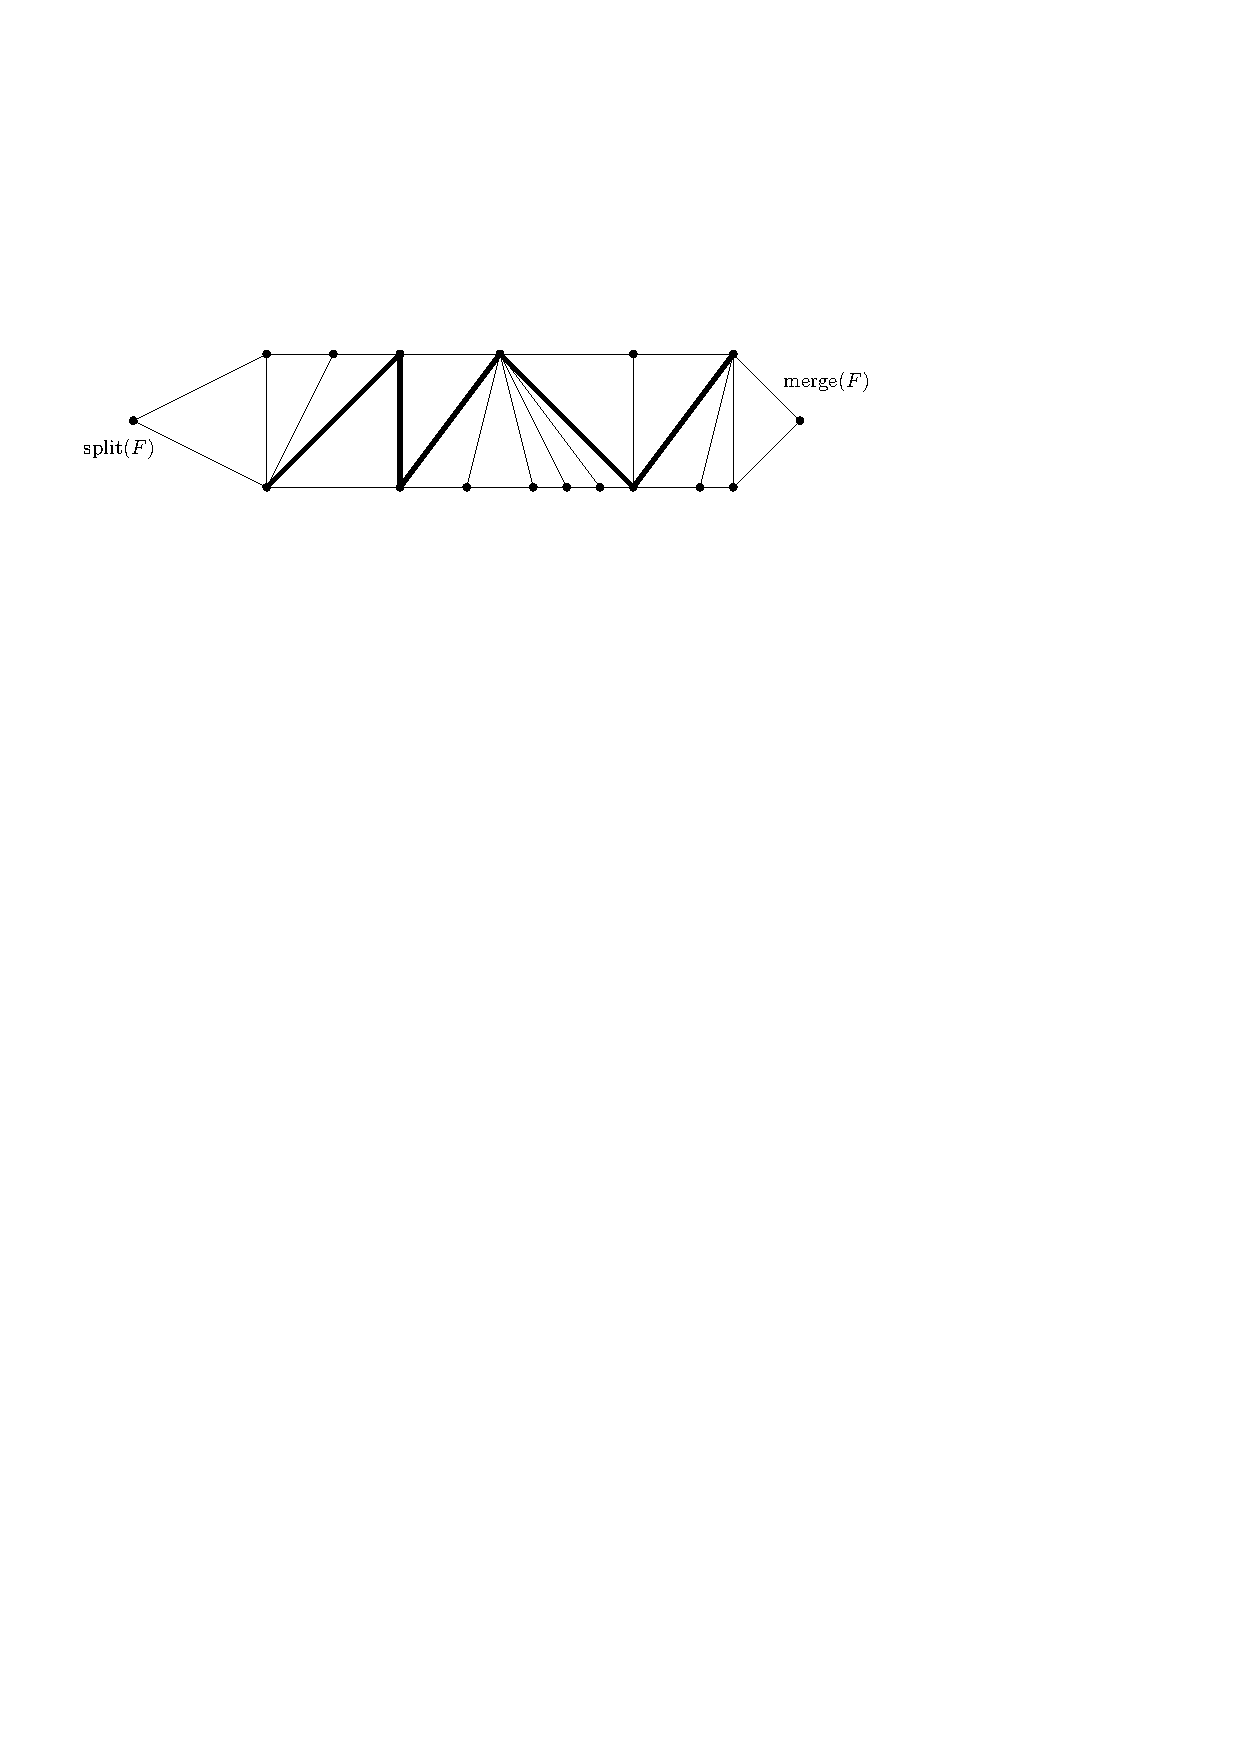
\includegraphics[scale=.9]{rectangularDuals/img/fans}
       \caption{An example face with fans.}
       \label{fig:uni:fans}
     \end{figure}

     \begin{figure}[h]
       \centering
       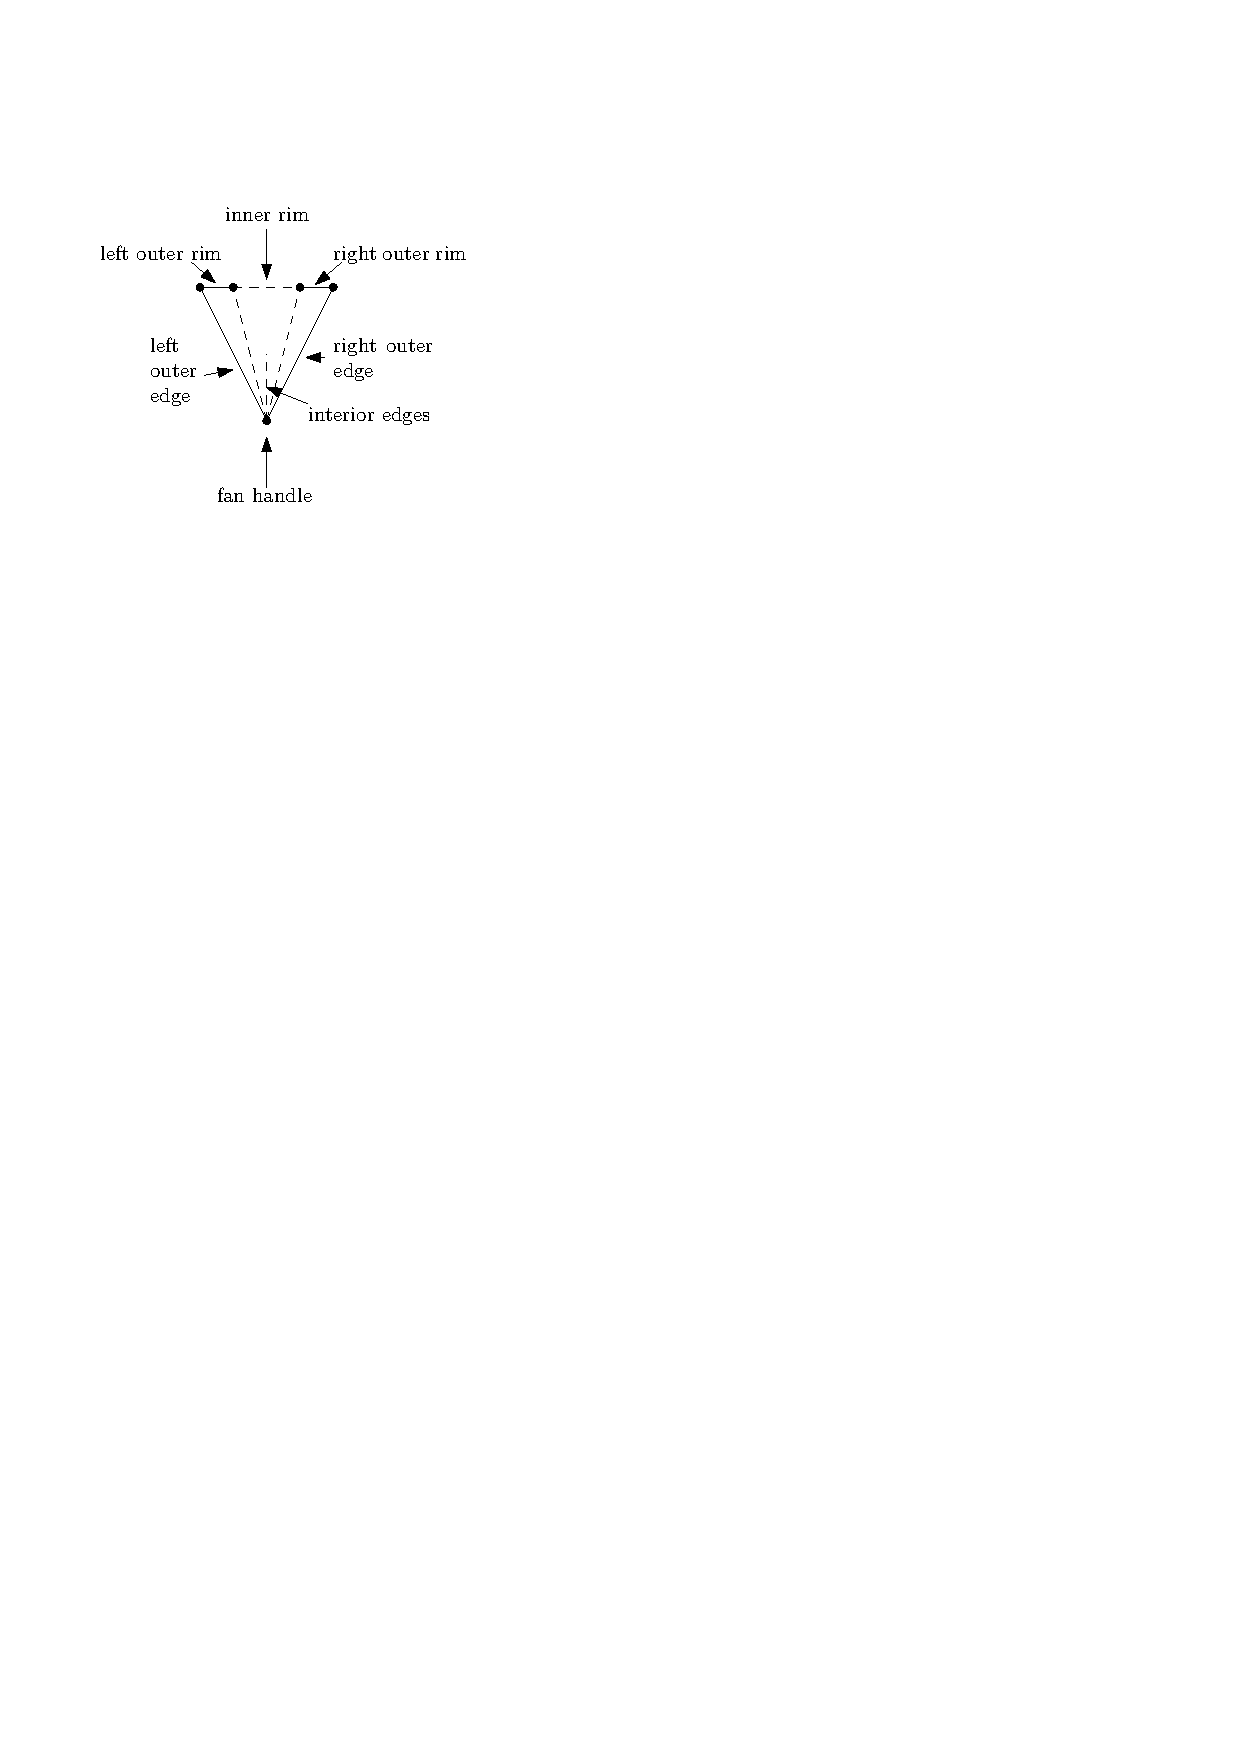
\includegraphics[scale=1]{rectangularDuals/img/fanterms}
       \caption{A number of fan-related terms.}
       \label{fig:rect:fanTerms}
     \end{figure}

\subsubsection{A useful property of this Regular edge labelling}
  Before finally discussing the property we will introduce two more definitions.
  A \emph{splitvertex} is a vertex with more than one outgoing blue edge.
  Given a splitvertex $v$ we will by \emph{bottom} path mean the path that comes in trough the first edge in the interval of incoming blue edges in the the rotation at $v$ and leaves through the last edge in the interval of outgoing blue edge in the rotation at $v$.
  See Figure \ref{fig:sweep:bottomPath}.

  \begin{figure}[h]
    \centering
    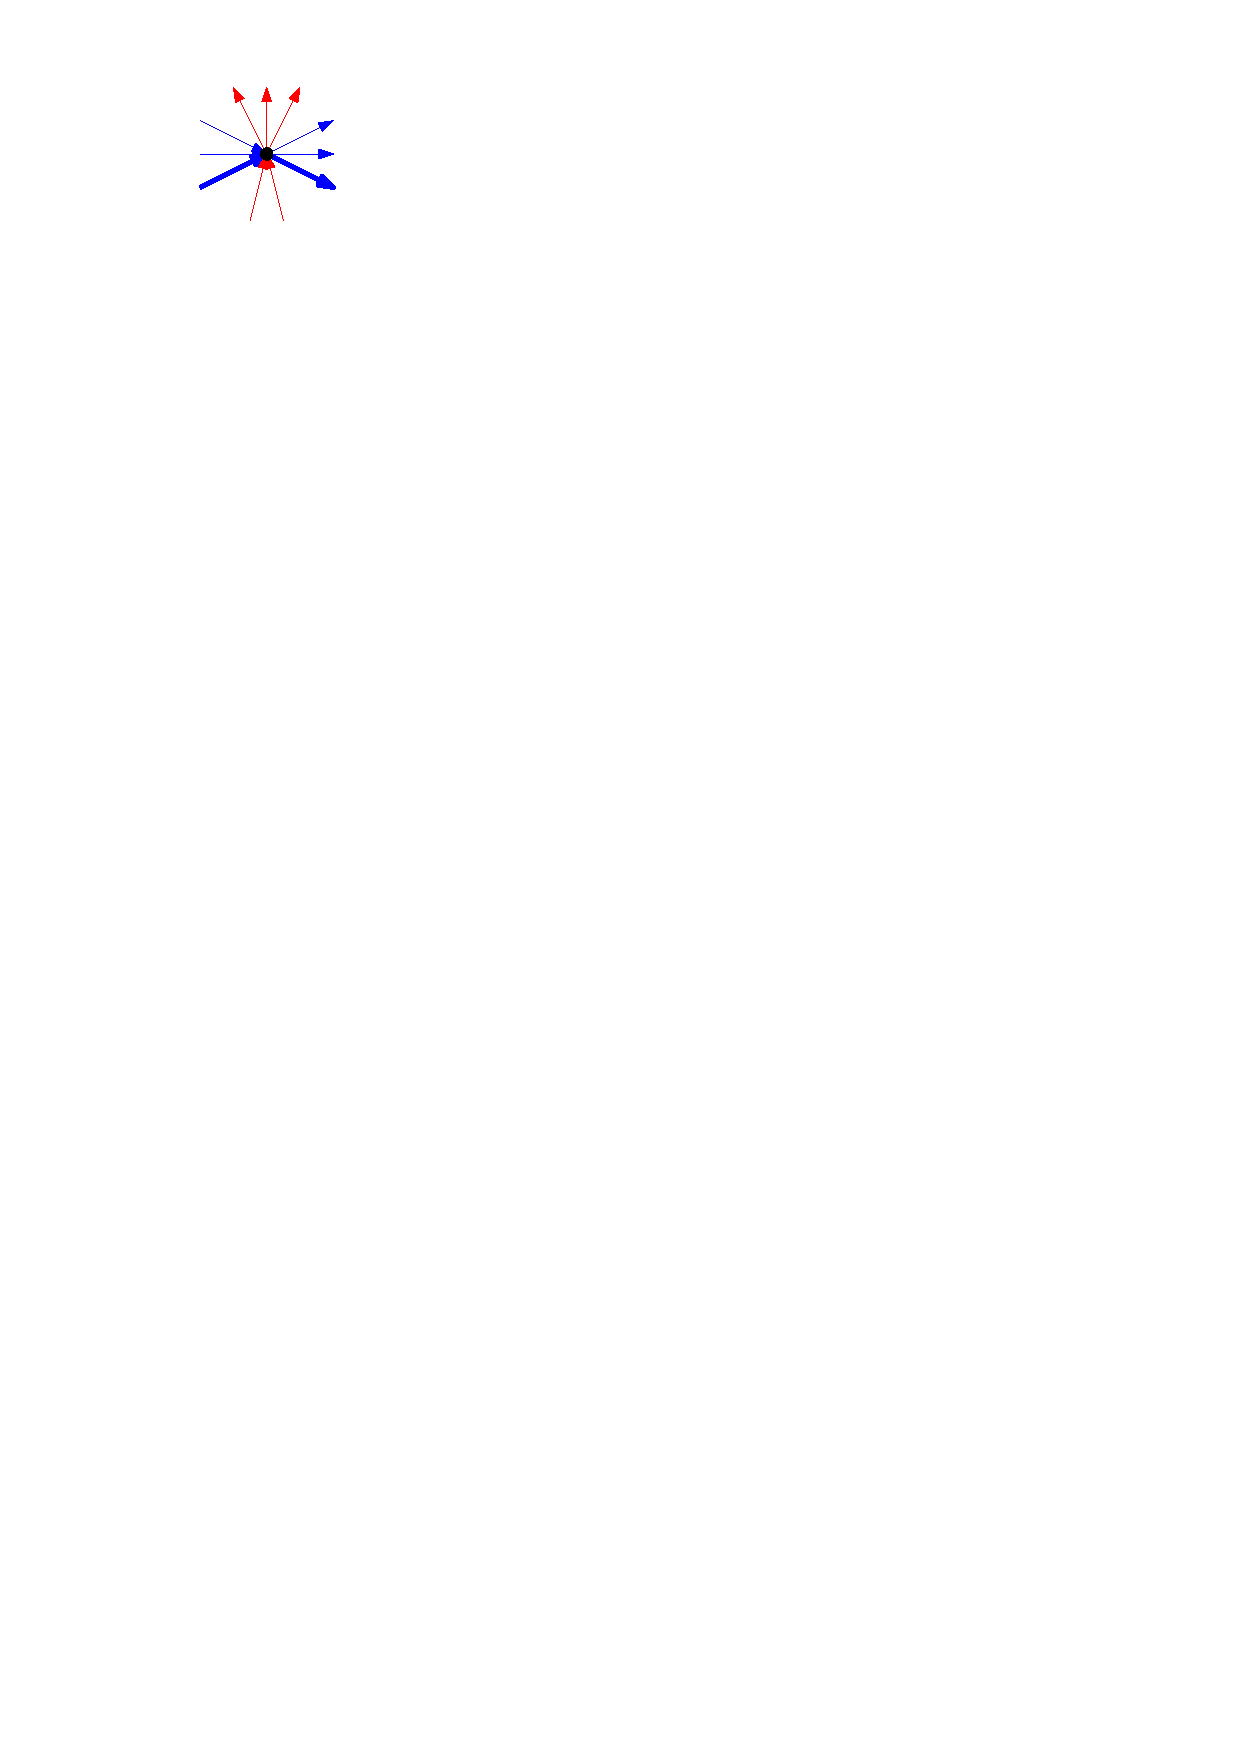
\includegraphics[scale=1]{unifiedAlgo/img/sweep/bottompath.pdf}
    \caption{The bottom path of this splitvertex is given in bold.}
    \label{fig:sweep:bottomPath}
  \end{figure}

  \begin{lemma}
    \label{lm:sweep:NoTwoSplitsAboveEachOther}
    Let $v$ be any splitvertex. Then the subsequent vertex on the bottom path $w$ can not be the handle of a large topfan.
  \end{lemma}

  \begin{proof}
    Note that if $v$ is a splitvertex because it is adjacent to $\pS$ then since $w$ is on the bottom path it also has to be adjacent to $\pS$ by the definition of the bottom path.
    Hence $w$ is not the handle of a large topfan in this case.

    On the other hand if $v$ is a splitvertex due to a chord $v a b x$ we can continue the bottom path past $w$ as an bottom path that will eventually go to $x$.
    Since every chord is evaded by a single path from $v_k$ to $v_\ell$ in the algorithm.
    We will denote this extended bottom path by $\P$.
    The situation is depicted in Figure \ref{fig:sweep:botomPathChord}.

    \begin{figure}[h]
      \centering
      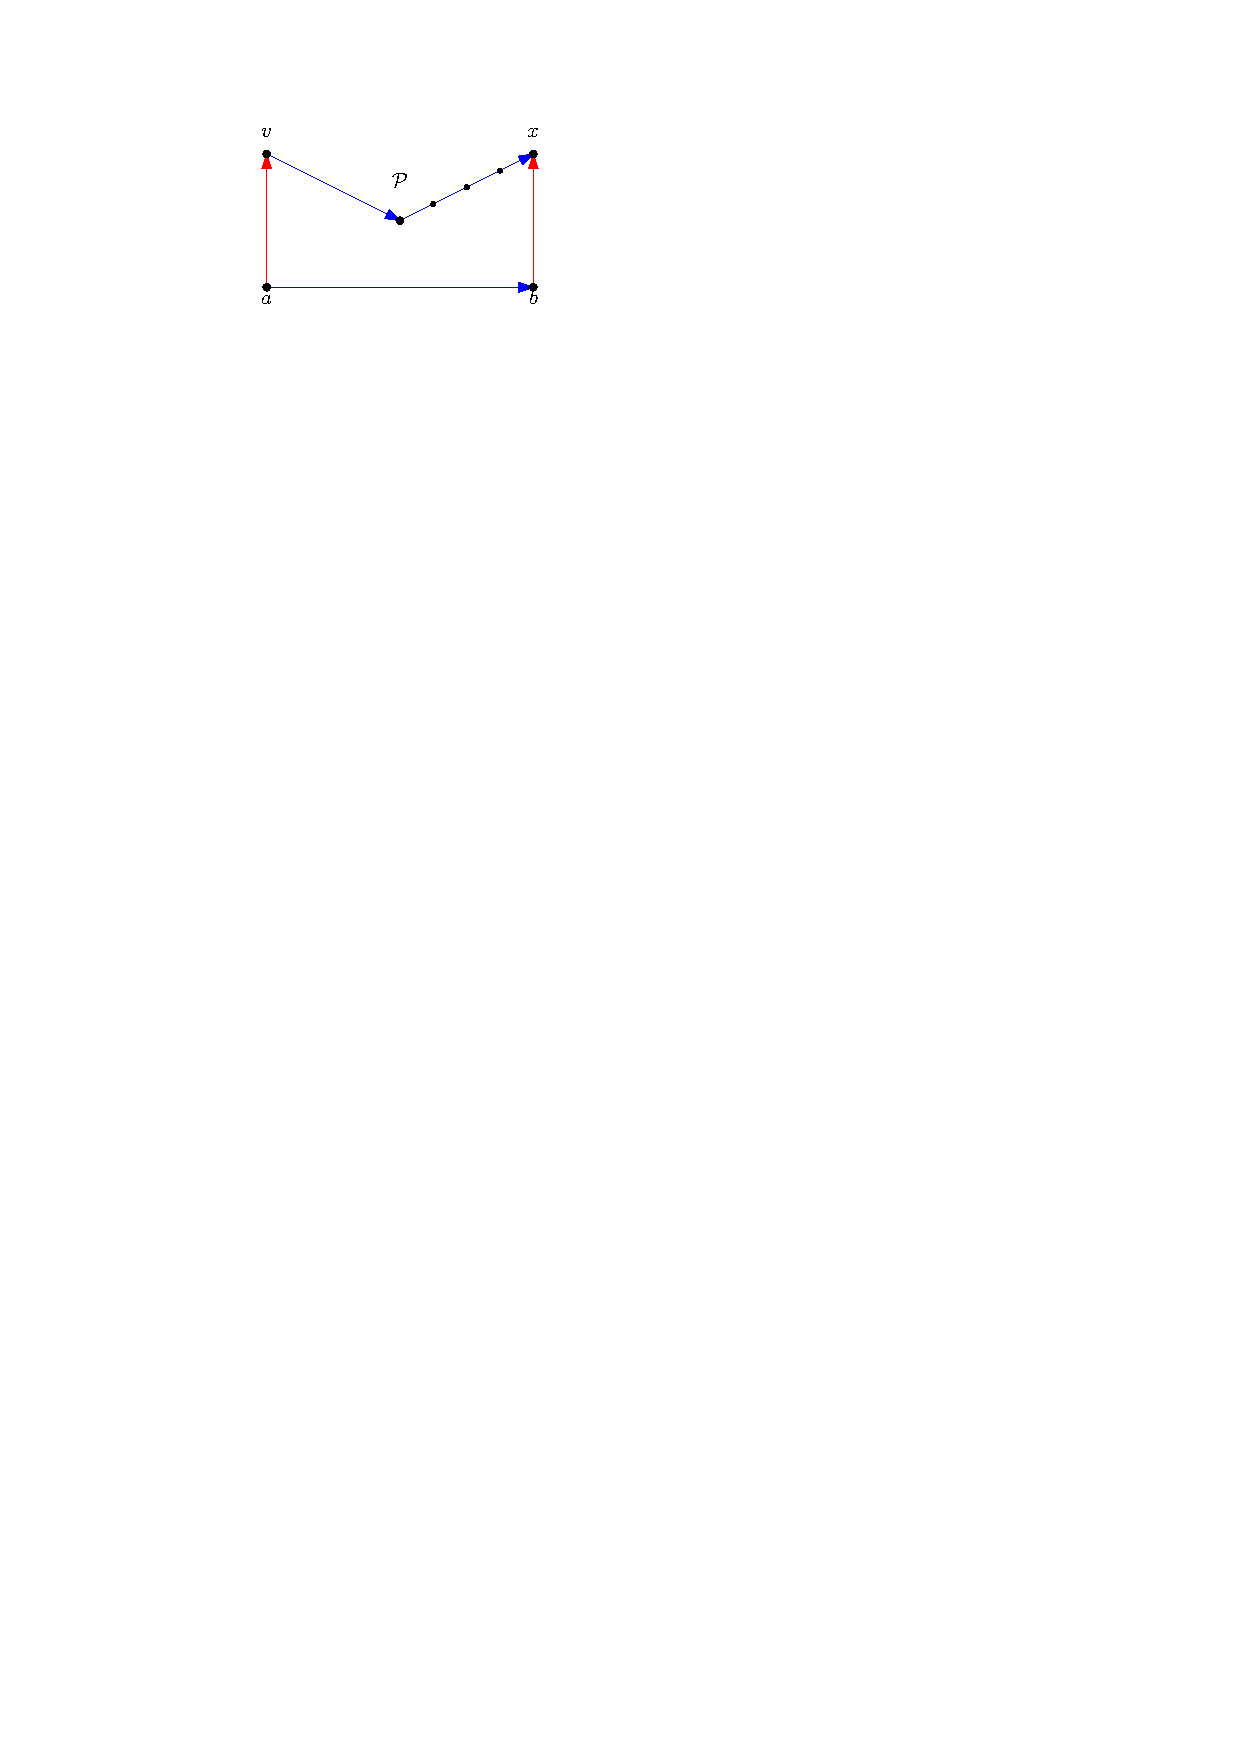
\includegraphics[scale=1]{unifiedAlgo/img/sweep/bottompathChord.pdf}
      \caption{The situation in the proof of Lemma \ref{lm:sweep:NoTwoSplitsAboveEachOther}}
      \label{fig:sweep:botomPathChord}
    \end{figure}

    The interior of  $vabx \oplus \rev \P$ and has no vertices. Suppose there would be such a vertex then since $\P$ is a bottom path the blue path going trough this vertex has to start at $a$ and end at $b$. But then this gives a blue face with only one edge on its bottom boundary path, hence the interior of this face has no incoming red edges.
    Which is impossible as can be seen in Figure \ref{fig:sweep:noFaceWithOneBottomEdge}.

    \begin{figure}[h]
      \centering
      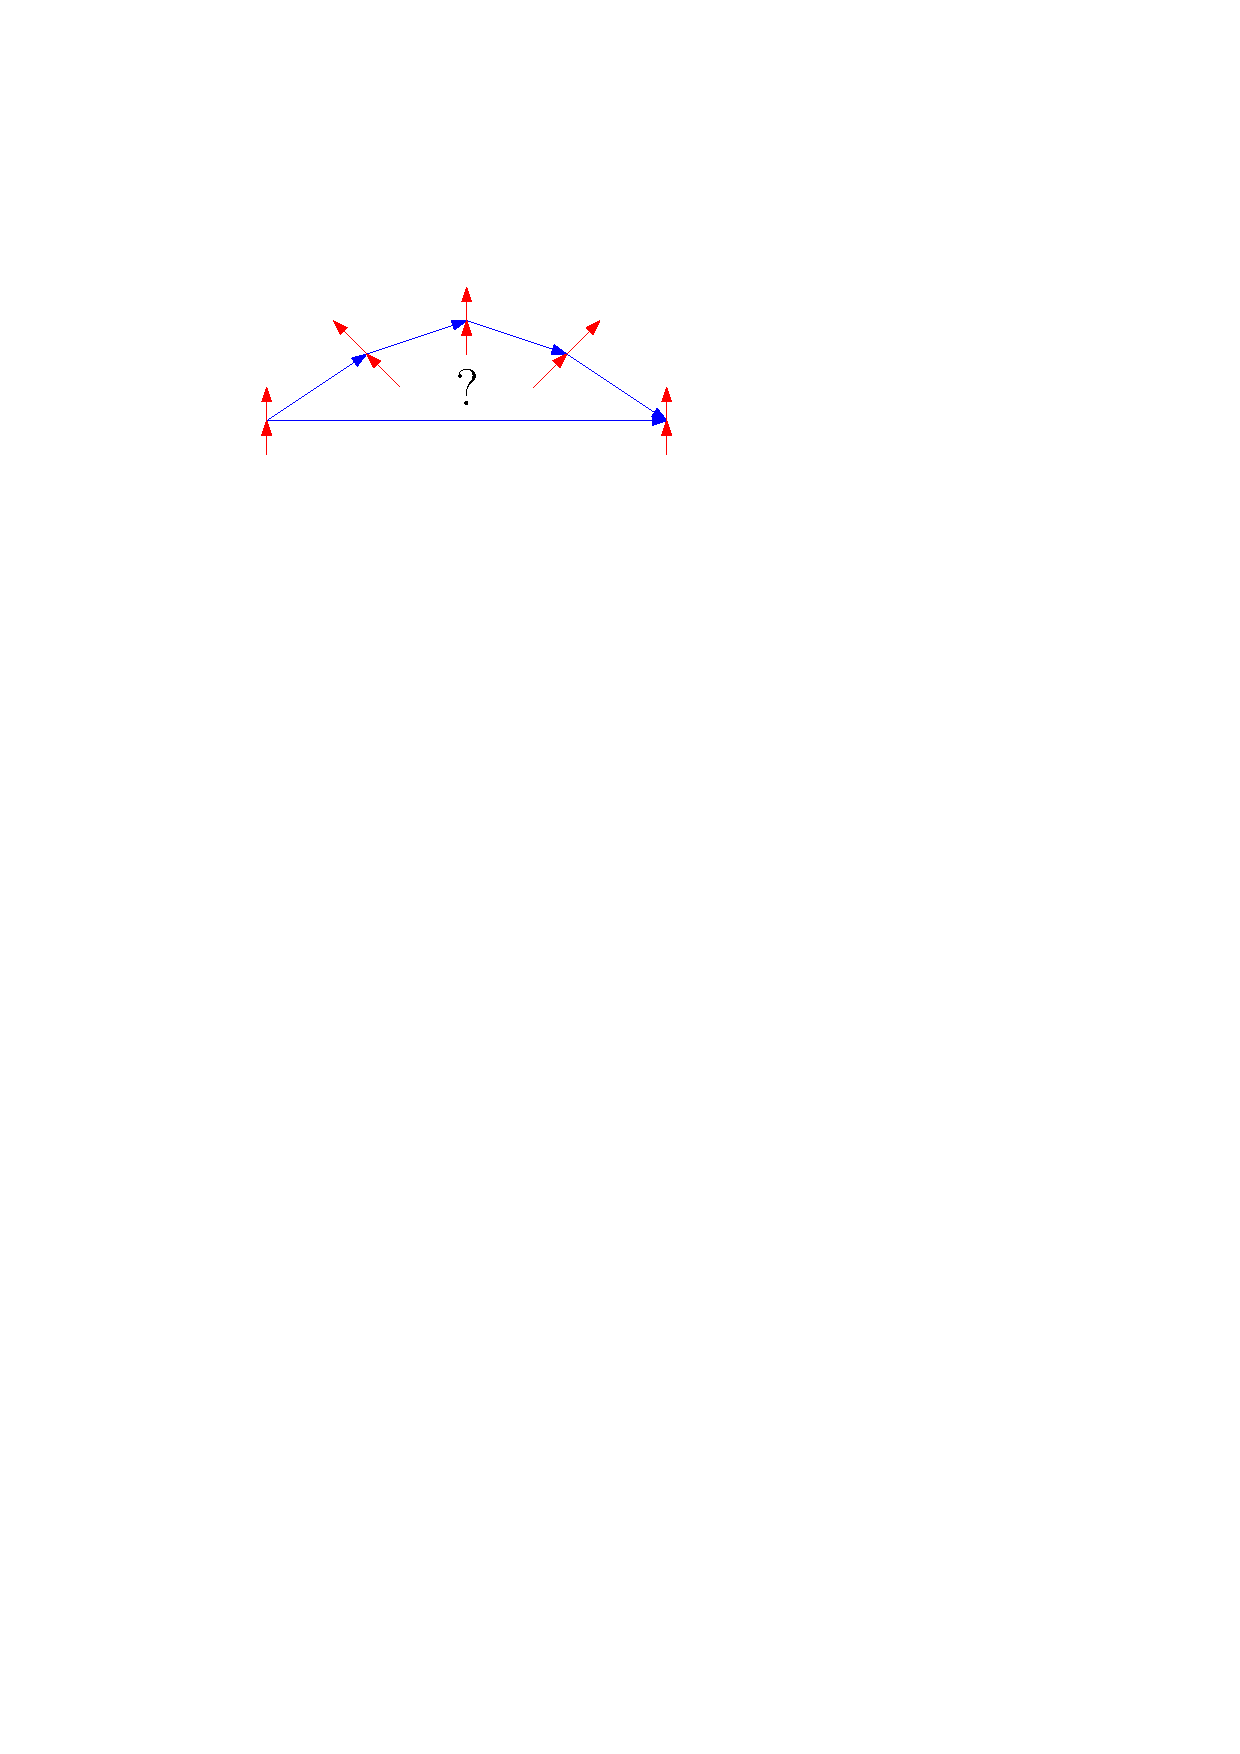
\includegraphics[scale=1]{unifiedAlgo/img/sweep/noFaceWithOneBottomEdge.pdf}
      \caption{The hypothetical situation of a face with bottom boundary path of length one.}
      \label{fig:sweep:noFaceWithOneBottomEdge}
    \end{figure}

    So the result is not a regular edge labeling. Since our graph is a regular edge labeling $vabx \oplus \rev \P$ has no interior vertices.

    This also implies all interior edges are red (by the definition of bottom path) and thus that $ab$ is blue otherwise we would get a monochromatic triangle.

    Now $w$ can not be connected to any vertex in $\P$ since that would imply the sweepcycle had a chord at some point.
    So $w$ can only be connected to $a$ and $b$ and is thus a topfan of size at most $2$.
    (If it is a topfan at all, since we do not consider topfans of size 1 as topfans.)
  \end{proof}
